\chapter{Value}
\lbl{ch:value}
\index{value}

\begin{quote}
Quite apart from many theoretical and practical problems that continue to
affect the species concept and its application, is it appropriate for
conservation\index{conservation} purposes to regard all species as equal in
this manner?  To a conservationist, regardless of relative abundance, is
\emph{Welwitschia}\index{Welwitschia@\emph{Welwitschia}} equal to a species
of \emph{Taraxacum}?\index{Taraxacum@\emph{Taraxacum}} Is the
panda\index{panda} equivalent to one species of rat?\index{rat}\\ 
\ \quad%
%
\index{Vane-Wright, Richard}
%
\hfill -- Vane-Wright et al.~(\cite{VWHW}, p.~237)
\end{quote}

\noindent
Putting aside entropy and diversity, let us consider a very
general question:
% 
\begin{quote}
\emph{What is the value of the whole in terms of its parts?}
\end{quote}
% 
Although the question in this form is far too vague to admit a mathematical
treatment, we will see that once posed precisely, it has a complete answer.
From that answer, the concept of diversity arises automatically.  The
answer also leads to a unique characterization of the Hill numbers (or
equivalently, the R\'enyi entropies), more powerful than the
characterization theorem in Section~\ref{sec:hill-char-given}.

We will consider a `whole' divided into $n$ `parts' of relative sizes $p_1,
\ldots, p_n$, which are assigned values $v_1, \ldots, v_n$ respectively
(Figure~\ref{fig:value}).
% 
\begin{figure}
\centering
\lengths
\begin{picture}(120,24)
\thicklines
\cell{60}{12}{c}{\includegraphics[height=24\unitlength]{value_simplem}}
\cell{30}{10}{c}{$p_1$}
\valput{34}{6}{$v_1$}
\cell{40}{18}{c}{$p_2$}
\valput{46}{15}{$v_2$}
\cell{49}{7.5}{c}{$p_3$}
\valput{54}{4.5}{$v_3$}
\cell{73}{10}{c}{$p_4$}
\valput{79}{7}{$v_4$}
\cell{80}{19}{c}{$p_5$}
\valput{86}{16}{$v_5$}
\end{picture}
\caption{A whole divided into $5$ parts, with relative sizes $(p_1, \ldots,
  p_5) \in \Delta_5$ and values $(v_1, \ldots, v_5)$.}
\lbl{fig:value}
\end{figure}
% 
The question is how to aggregate those values into a
single value $\sigma(\p, \vc{v})$ for the whole, measured in the same units
as the values $v_i$ of the parts.  This aggregation method should have
sensible properties.  For instance, if we put together two parts of equal
size and equal value, $v$, the result should have value $2v$.  

One simple method is to ignore the sizes of the parts and just sum their
values, so that
\[
\sigma(\p, \vc{v}) = v_1 + \cdots + v_n
\]
(or better, $\sigma(\p, \vc{v}) = \sum_{i \in \supp(\p)} v_i$).  But there
are many other possibilities.  In fact, we will define a one-parameter
family $(\sigma_q)$ of value measures.  They include as special cases the
Hill numbers $D_q$, the more general similarity-sensitive diversity
measures $D_q^Z$ of Chapter~\ref{ch:sim}, certain phylogenetic diversity
measures (due to Chao, Chiu and Jost~\cite{CCJ}), and, essentially, the
$\ell^p$\index{pnorm@$p$-norm} norms.  For example, when a community is
divided into $n$ species in proportions $p_1, \ldots, p_n$, and each
species is assigned the same value, $1$, the value of the whole according
to $\sigma_q$ is the Hill number of order $q$:
\[
\sigma_q\bigl(\p, (1, \ldots, 1)\bigr) = D_q(\p).
\]

In most of the cases just listed, the whole is taken to be an ecological
community and the parts are its species.  But there is an important
complementary situation, in which the whole is still a community but the
parts are taken to be subcommunities.  For instance, the community
might be divided geographically into regions, and we might attempt to
evaluate the community as a whole based on the sizes and values of those
regions.  In the case where value is interpreted as diversity, that is
exactly what we did when we derived the chain rule for diversity
(Propositions~\ref{propn:hill-chn} and~\ref{propn:div-sim-ch}).  Indeed,
the function $\sigma_q$ can be seen as an embodiment of the chain rules for
$D_q$ and $D_q^Z$, in a sense explained in Example~\ref{eg:value-ch}.

We begin by defining the value measures $\sigma_q$ and analysing some
special cases (Section~\ref{sec:value-defn}), with important examples from
both ecology and the analysis of social welfare.  We then introduce the
R\'enyi relative entropies, which are very closely related to the value
measures $\sigma_q$.  (The $q$-logarithmic relative entropies were already
covered in Section~\ref{sec:q-log-ent}.)  As a bonus, we use the R\'enyi
and $q$-logarithmic relative entropies to provide further evidence for the
canonical nature of the Fisher metric on probability distributions
(Remark~\ref{rmks:fisher-def}\bref{rmk:fisher-def-gods-joke}).

Using our earlier results on means, we then prove that the only value
measures with reasonable properties are those belonging to the family
$(\sigma_q)$ (Section~\ref{sec:value-char}).  From this we deduce that for
communities modelled as their relative abundance distributions,
the only reasonable measures of diversity are the Hill numbers
(Section~\ref{sec:total-hill}).

We have already proved a characterization theorem for the Hill%
%  
\index{Hill number!difference between characterizations of}
% 
numbers $D_q$ in Section~\ref{sec:hill-char-given}, showing that for a
\emph{fixed} $q$, if a diversity measure $D$ has certain properties
\emph{depending on $q$}, then it must be equal to $D_q$.  But in the
theorem proved in this chapter, there is no `$q$' mentioned in the
hypotheses, and the conclusion is that $D$ must be equal to $D_q$
\emph{\,for some $q$}.  In short, the earlier theorem characterized
the Hill numbers individually, but this theorem characterizes them as a
family.


\section{Introduction to value}
\lbl{sec:value-defn}


Here we consider sequences of functions
\[
\bigl( 
\sigma \from \Delta_n \times [0, \infty)^n \to [0, \infty) 
\bigr)_{n \geq 1},
\]
which will be referred to as \demph{value%
%
\index{value measure}
%
measures}.  We regard a pair $(\p, \vc{v}) \in \Delta_n \times [0,
\infty)^n$ as representing a whole made up of $n$ disjoint parts with
relative sizes $p_1, \ldots, p_n$ and values $v_1, \ldots, v_n$, and we
regard $\sigma(\p, \vc{v})$ as the value that $\sigma$ assigns to the
whole.

A special role is played by the family 
\[
\bigl( \sigma_q \bigr)_{q \in [-\infty, \infty]}
\ntn{sigmaq}
\]
of value\index{value measure} measures, defined by
\[
\sigma_q(\p, \vc{v}) = M_{1 - q} (\p, \vc{v}/\p)
\]
($n \geq 1$, $\p \in \Delta_n$, $\vc{v} \in [0, \infty)^n$).  The
convention adopted in Remark~\ref{rmk:defined-even-if-not} ensures that
$\sigma_q(\p, \vc{v})$ is always well-defined.
We call $\sigma_q$ the \demph{value measure of order~%
%
\index{value measure!order q@of order $q$}%
\index{order!value measure@of value measure}
%
$q$}.  Explicitly, when $q \neq 1, \pm \infty$,
\[
\sigma_q(\p, \vc{v})
=
\Biggl( 
\sum_{i \in \supp(\p)} p_i^q v_i^{1 - q} 
\Biggr)^{1/(1 - q)},
\]
unless $q > 1$ and $v_i = 0$ for some $i \in \supp(\p)$, in which case
$\sigma_q(\p, \vc{v}) = 0$.  For $q \in \{1, \pm\infty\}$, 
% 
\begin{align*}
\sigma_{-\infty}(\p, \vc{v})    &
=
\max_{i \in \supp(\p)} \frac{v_i}{p_i}, \\
\sigma_1(\p, \vc{v})    &
=
\prod_{i \in \supp(\p)} \biggl( \frac{v_i}{p_i} \biggr)^{p_i},    \\
\sigma_{\infty}(\p, \vc{v})     &
=
\min_{i \in \supp(\p)} \frac{v_i}{p_i}.
\end{align*}
% 

\begin{examples}
\lbl{egs:val-first}
\begin{enumerate}
\item 
\lbl{eg:val-first-indivs} 
Consider a set of $k$ individuals, divided into $n$ equivalence classes
(`parts'), with the $i$th part consisting of $k_i$ individuals.  Let $p_i =
k_i/k$ be the proportion of individuals in the $i$th part.  Let $v_1,
\ldots, v_n \in [0, \infty)$ be any values assigned to the parts.  Then
\[
\sigma_q(\p, \vc{v})
=
M_{1 - q}\Biggl( 
\p, \Biggl( \frac{kv_1}{k_1}, \ldots, \frac{kv_n}{k_n} \Biggr)
\Biggr),
\]
or equivalently,
% 
\begin{equation}
\lbl{eq:val-indivs}
\sigma_q(\p, \vc{v})
=
k \cdot 
M_{1 - q}\Biggl( 
\p, \Biggl( \frac{v_1}{k_1}, \ldots, \frac{v_n}{k_n} \Biggr)
\Biggr).
\end{equation}
% 
This can be understood as follows.  If the value $v_i$ of the $i$th part is
shared out evenly among its $k_i$ members, then the value%
%
\index{value!per individual}
% 
per individual in the $i$th part is $v_i/k_i$.  Hence the mean value per
individual in the whole is
\[
M_{1 - q}\Biggl(
\p, \Biggl( \frac{v_1}{k_1}, \ldots, \frac{v_n}{k_n} \Biggr)
\Biggr).
\]
So, equation~\eqref{eq:val-indivs} states that
% 
\[
\text{value of whole} = \text{number of individuals}
\times \text{mean value per individual}.
\]
% 
This is the basic conceptual relationship between value measures and
means. 

\item
If in~\bref{eg:val-first-indivs} we interpret `mean' as arithmetic mean,
then we are in the case $q = 0$, and $\sigma_0$ is simply given by
\[
\sigma_0(\p, \vc{v}) = \sum_{i \in \supp(\p)} v_i
\]
(as in the introduction to this chapter).  But we have seen repeatedly in
this book that the \emph{arithmetic} mean is not the only useful kind.  The
other power means should always be considered alongside it, and in this
case, they give the whole family $(\sigma_q)$. 
\end{enumerate}
\end{examples}

\begin{remark}
\lbl{rmk:vals-mns}
The value measures $\sigma_q$ and the power means $M_t$ are sequences of
functions of the same type:
\[
\bigl( 
\sigma_q, M_t \from \Delta_n \times [0, \infty)^n \to [0, \infty)
\bigr)_{n \geq 1}.
\]
However, Example~\ref{egs:val-first}\bref{eg:val-first-indivs} makes clear
that there should be no overlap%
%
\index{value measure!mean@vs.\ mean}%
\index{mean!value measure@vs.\ value measure}
% 
between the classes of value measures and means.  Indeed, a reasonable
value measure $\sigma$ should satisfy
\[
\sigma\bigl( \vc{u}_n, (v, \ldots, v)\bigr) = nv,
\]
whereas a minimal requirement of a mean $M$ is the consistency condition
\[
M\bigl( \vc{u}_n, (x, \ldots, x)\bigr) = x.
\]
So, no reasonable mean is a reasonable value measure.  We return to the
relationship between means and value measures in
Section~\ref{sec:value-char}.
\end{remark}

For positive parameters $q$, the value of the whole is never more than the
sum of the values of its parts:

\begin{lemma}
\lbl{lemma:sigma-sum-ineq}
For all $q \geq 0$, $\p \in \Delta_n$, and $\vc{v} \in [0, \infty)^n$,
\[
\sigma_q(\p, \vc{v}) \leq \sum_{i = 1}^n v_i.
\]
For $q > 0$, equality holds if and only if $\vc{v}$ is a scalar multiple of
$\p$.
\end{lemma}

So for fixed $\sum v_i$, the value of the whole is maximized when value
is spread evenly across the constituent parts, in proportion to their
sizes.

\begin{proof}
For all $q \geq 0$,
\[
\sigma_q(\p, \vc{v})    
=
M_{1 - q}(\p, \vc{v}/\p)        
\leq
M_1(\p, \vc{v}/\p) 
=
\sum_{i \in \supp(\p)} v_i      
\leq
\sum_{i = 1}^n v_i.
\]
Assuming now that $q > 0$, equality holds in the first inequality if and
only if $v_i/p_i$ is constant over $i \in \supp(\p)$ (by
Theorem~\ref{thm:mns-inc-ord}), and in the second if and only if $v_i = 0$
for all $i \not\in \supp(\p)$.  The result follows.
\end{proof}

The next two examples illuminate the meaning of the parameter $q$.
They concern the case where the parts are of equal size ($\p = \vc{u}_n$),
so that the value measures $\sigma_q$ are given by
\[
\sigma_q(\vc{u}_n, \vc{v}) = n \cdot M_{1 - q}(\vc{u}_n, \vc{v})
\]
($q \in [-\infty, \infty]$, $\vc{v} \in [0, \infty)^n$).  

\begin{example}
A classical question in welfare%
%
\index{welfare}
%
economics%
% 
\index{economics} 
% 
is how to take a group
of agents, each of which has an assigned utility,%
% 
\index{utility}
% 
and aggregate their individual utilities into a measure of the utility of
the group as a whole.  For instance, the agents might be the citizens of a
society, and the utility of a citizen might be their individual level of
welfare, wealth or well-being.  The challenge, then, is to combine them
into a single number representing the collective welfare of the society.
(As a general reference for all of this example, we refer to Section~1.2
and Chapter~3 of Moulin~\cite{Moul}.)
% , with references in Section~3.7.  

Specifically, fix $n$, and take a group of $n$ individuals with respective
utilities $v_1, \ldots, v_n \geq 0$.  A \demph{collective%
% 
\index{collective utility function} 
% 
utility function} assigns a real number $f(\vc{v})$ to each such tuple
$\vc{v} = (v_1, \ldots, v_n)$.  
For example,
\[
\sigma_q(\vc{u}_n, -) \from [0, \infty)^n \to \R
\]
is a collective utility function for each $q \in [-\infty, \infty]$.  

More important than the collective utility function $f$ itself is its
associated \demph{social% 
%
\index{social welfare function}%
\index{ordering, social welfare}
%
welfare ordering}, which is the relation $\swo$ on $[0, \infty)^n$ defined
  by
\[
\vc{v} \swo \vc{v}' \iff f(\vc{v}) \leq f(\vc{v}').
\]
In the case of the welfare of the citizens of a society, $\vc{v} \swo
\vc{v}'$ is interpreted as the judgement that when the welfare levels of
the citizens are $v_1, \ldots, v_n$, society is in a poorer state than when
they are $v'_1, \ldots, v'_n$.

Of course, such judgements depend on a choice of collective utility
function $f$.  When $f = \sigma_q(\vc{u}_n, -)$, different values of $q$
correspond to different viewpoints, some of which are associated with
particular schools of political% 
%
\index{politics} 
%
philosophy.%
% 
\index{philosophy, political}
% 
The case $q = 0$ is
\[
\sigma_0(\vc{u}_n, -) \from 
\vc{v} \mapsto \sum v_i,
\]
so that the collective welfare is simply the sum of the individual welfares.
This function is associated with classical utilitarianism,%
% 
\index{utilitarianism} 
%
with its
roots in the philosophy of Jeremy Bentham%
% 
\index{Bentham, Jeremy} 
%
and in John Stuart Mill's%
% 
\index{Mill, John Stuart}
%
`sum total of happiness'.  When $q = \infty$, the collective utility
function is
\[
\sigma_\infty(\vc{u}_n, -) \from
\vc{v} \mapsto n \min v_i,
\]
so that
\[
\vc{v} \swo \vc{v}' \iff \min v_i \leq \min v'_i.
\]
This viewpoint on collective welfare is associated with the philosophy of
John Rawls:%
%
\index{Rawls, John}
% 
a society should be judged by the welfare of its most
miserable citizen.  An intermediate position is $q = 1$, where
\[
\sigma_1(\vc{u}_n, -) \from 
\vc{v} \mapsto n \cdot \biggl( \prod v_i \biggr)^{1/n}
\]
and so
\[
\vc{v} \swo \vc{v}' \iff \prod v_i \leq \prod v'_i.
\]
In this context, the product operation $\vc{v} \mapsto \prod v_i$ is known
as the \demph{Nash%
% 
\index{Nash collective utility function} 
% 
collective utility function}, and has special properties not shared by any
other collective utility function (unsurprisingly, given the special role
played by the case $q = 1$ in the context of entropy).
% Chapter~3 of Moulin~\cite{Moul} provides details on all of the above, with 
% references in Section~3.7.

An important property of collective utility functions is the
Pigou--Dalton%
% 
\index{Pigou--Dalton principle}
% 
principle.  In the language of wealth, this states that transferring a
small amount of wealth from a richer citizen to a poorer one is beneficial
to the overall welfare of society.  Formally, let $\vc{v} \in [0,
  \infty)^n$ and $i, j \in \{1, \ldots, n\}$ with $v_i < v_j$, and let $0
  \leq \delta \leq (v_j - v_i)/2$; define $\vc{v}' \in [0, \infty)^n$ by
\[
v'_k =
\begin{cases}
v_i + \delta &\text{if } k = i,      \\
v_j - \delta &\text{if } k = j,      \\
v_k     &\text{otherwise}.
\end{cases}
\]
The \demph{Pigou--Dalton principle} is that $\vc{v} \swo \vc{v'}$ for
all such $\vc{v}$, $i$, $j$, and $\delta$.

When $q \in [0, \infty]$, an elementary calculation shows that
$\sigma_q(\vc{u}_n, -)$ satisfies the Pigou--Dalton principle.  Thus,
redistribution%
% 
\index{redistribution of wealth} 
% 
is regarded positively.  On the other hand, the Pigou--Dalton principle
fails for all $q \in [-\infty, 0)$.  In fact, for $q \in (-\infty, 0)$,
  redistribution from richer to poorer always strictly \emph{decreases}
  overall welfare.  In the extreme case $q = -\infty$, the collective
  utility function is
\[
\sigma_{-\infty}(\vc{u}_n, -) \from \vc{v} \mapsto n \max_i v_i,
\]
so that the welfare of a society is proportional to the welfare of its most
privileged citizen.  (Recall that $n$ is fixed.)  Thus, from the viewpoint
of $q = -\infty$, collective welfare is optimized when all the wealth is
transferred to a single individual.  In the welfare economics literature,
negative values of $q$ are often excluded.

(The family $(\sigma_q(\vc{u}_n, -))$ of collective utility functions that
we have used is different from the family used in economics texts such as
Moulin~\cite{Moul}, but only superficially.  In the literature, it is
conventional to use the functions
\[
\begin{array}{rcll}
\vc{v}  &\mapsto        &\sum v_i^t     &(t \in (0, \infty)),   \\
\vc{v}  &\mapsto        &\sum \log v_i,         &               \\
\vc{v}  &\mapsto        &-\sum v_i^t  &(t \in (-\infty, 0)),
\end{array}
\]
whereas we have been using
% 
\begin{equation}
\lbl{eq:val-ufm-exp}
\vc{v} \mapsto \sigma_q(\vc{u}_n, \vc{v})
=
\begin{cases}
n^{q/(q - 1)} \Bigl( \sum v_i^{1 - q} \Bigr)^{1/(1 - q)}      &
\text{if } 1 \neq q \in (-\infty, \infty),      \\
n \prod v_i^{1/n}       &
\text{if } q = 1.
\end{cases}
\end{equation}
% 
But reparametrizing with $q = 1 - t$, the induced social welfare orderings
are identical.)
\end{example}

\begin{example}
In contexts such as collective welfare and diversity, it is natural to
restrict the parameter $q$ to be positive.  But for negative parameters
$q$, the value measures $\sigma_q$ also define something important, at
least when the parts are of equal size: the $\ell^p$\index{pnorm@$p$-norm}
norms.  Indeed, for $-\infty < q \leq 0$, equation~\eqref{eq:val-ufm-exp}
gives
\[
\sigma_q(\vc{u}_n, \vc{v})      
=
n^{q/(q - 1)} \|\vc{v}\|_{1 - q},
\]
where the norm $\|\cdot\|_{1 - q}$ is as defined in
Example~\ref{eg:norm-p}.
\end{example}

We now show that all of the diversity measures discussed in
previous chapters are encompassed by the value measures $\sigma_q$.

\begin{example}
\lbl{eg:value-hill}
Consider an ecological community made up of species with relative abundances
$p_1, \ldots, p_n$.  In the absence of other information, it is
natural to give all the species the same value, $1$.  We have
\[
\sigma_q\bigl( \p, (1, \ldots, 1)\bigr)
=
M_{1 - q}(\p, 1/\p)
=
D_q(\p),
\]
so the value assigned to the community by $\sigma_q$ is the Hill
number $D_q(\p)$.
\end{example}

\begin{example}
\lbl{eg:value-dqz} 
Now let us enrich our model of the community with an $n \times n$
similarity matrix $Z$.  Assume that the diagonal entries of $Z$ are all $1$
(as discussed on p.~\pageref{p:Z1}).  Based on this model, what value $v_i$
can we 
reasonably assign to each species?

In Section~\ref{sec:sim-basic}, we considered the quantity 
\[
(Z\p)_i
=
\sum_{j = 1}^n Z_{ij} p_j
\]
associated with the $i$th species.  This is the expected similarity between
an individual of species $i$ and an individual chosen from the community at
random.  We called $(Z\p)_i$ the ordinariness of species $i$, and
$1/(Z\p)_i$ its specialness.%
%
\index{specialness}  

This might seem to suggest using $1/(Z\p)_i$ as the value of the $i$th
species.  However, $1/(Z\p)_i$ is a measure of the specialness of an
\emph{individual} of the $i$th species, whereas $v_i$ is supposed to
measure the value of the $i$th part (species) \emph{as a whole}.  We
therefore define $v_i$%
%
\index{value!species@of a species}
%
to be the specialness per individual
in the species multiplied by the size of the species:
\[
v_i 
=
\frac{p_i}{(Z\p)_i}.
\]
When $Z$ is the naive similarity matrix $I$, this formula reduces to $v_i =
1$, as in Example~\ref{eg:value-hill}.  More generally, if species $i$ is
completely dissimilar to all other species ($Z_{ij} = 0$ for all $i \neq
j$) then $v_i = 1$.  In any case, $v_i \leq 1$, since $(Z\p)_i \geq p_i$ 
(inequality~\eqref{eq:Zpi-lb1}, p.~\pageref{eq:Zpi-lb1}).  Lower values
$v_i$ indicate that in comparison to the size of the $i$th species, there
are many individuals belonging to species similar to it.  This agrees with
the intuition that such a species contributes little to the diversity of
the whole.

With this definition of $\vc{v}$ as $\p/Z\p$, we recover the
similarity-sensitive diversity measures $D_q^Z$ of Chapter~\ref{ch:sim}:
\[
\sigma_q(\p, \p/Z\p)
=
M_{1 - q}(\p, 1/Z\p)
=
D_q^Z(\p),
\]
by definition of $D_q^Z$.
\end{example}

\begin{example}
\lbl{eg:value-ch} 
%
Now take a community of individuals that are not only classified into a
number of species (with similarities encoded in a matrix $Z$), but
also divided into $n$ disjoint subcommunities.  Thus, each individual
belongs to exactly one species and exactly one subcommunity.  We will
assume that the different subcommunities share no species, and that species
in different subcommunities are completely dissimilar (as in
Example~\ref{eg:div1-chain-islands} and Propositions~\ref{propn:hill-chn}
and~\ref{propn:div-sim-ch}, where the subcommunities were called
`islands').%
%
\index{islands!diversity of group of}

Write $w_i$ for the population size of the $i$th subcommunity relative to
the whole community, so that $\sum w_i = 1$.  Also write $d_i$ for the
diversity of order $q$ of the $i$th subcommunity.  Then by the chain rule
for the similarity-sensitive diversities
(Proposition~\ref{propn:div-sim-ch}), the diversity of order $q$ of the
whole community is
\[
\sigma_q(\vc{w}, \vc{d}).
\]
This is the fundamental relationship%
%
\index{value!diversity@and diversity}%
\index{diversity!value@and value}
% 
between value and diversity.  If value is taken to mean diversity of order
$q$, then $\sigma_q$ correctly aggregates the values of the parts of a
community to give the value of the whole.
\end{example}

\begin{example}
In the ecological settings discussed, we have only ever considered the
\emph{relative} abundances of species.  But absolute%
%
\index{abundance!absolute}
%
abundances sometimes matter.  What happens if we measure the value of a
species within a community as its absolute abundance?

Consider a community of individuals divided into $n$ species, with absolute
abundances $A_1, \ldots, A_n$.  Writing $A = \sum A_i$, the relative
abundances are $p_i = A_i/A$.  For all $q \in [-\infty, \infty]$,
% 
\begin{align*}
\sigma_q\bigl(\p, (A_1, \ldots, A_n)\bigr)      &
=
M_{1 - q}\Biggl( 
\p, \Biggl(\frac{A_1}{p_1}, \ldots, \frac{A_n}{p_n}\Biggr) 
\Biggr)  \\
&
=
M_{1 - q}\bigl( \p, (A, \ldots, A) \bigr)       \\
&
=
A.
\end{align*}
% 
So, the value of the whole is simply the total abundance.

In this example, the value measures $\sigma_q$ give us no interesting new
quantity.  The answer to the question posed is trivial.  But it is also
reasonable: if the value of each part of a community is taken to be just
the number of individuals it contains, it is natural that the value of the
whole community is measured in that way too.
\end{example}

We conclude this introduction to value with a more substantial example.

\begin{example}
\lbl{eg:value-ccj}
\index{phylogenetic!diversity}%
\index{Chao, Anne!Chiu--Jost@--Chiu--Jost phylogenetic diversity}
% 
Here we describe the phylogenetic diversity measures of Chao, Chiu and
Jost~\cite{CCJ} and show that they too are a special case of the value
measures $\sigma_q$.

A \demph{phylogenetic tree}\index{phylogenetic!tree} is a depiction of the
evolutionary history of a group of species, as in
Figure~\ref{fig:phylo-trees}.  (For a general guide to the subject, see
Lemey et al.~\cite{LSV}.)
% 
\begin{figure}
\centering
\lengths
\begin{picture}(44,57)(0,-2)
\cell{22.9}{55}{t}{\includegraphics[width=41.8\unitlength]{phylo-a}}
\cell{0}{28}{l}{\rotatebox{-90}{\normalsize time}}
\cell{6.5}{9}{b}{1}
\cell{11}{9}{b}{2}
\cell{15.6}{9}{b}{3}
\cell{20.1}{9}{b}{4}
\cell{24.7}{9}{b}{5}
\cell{29.2}{9}{b}{6}
\cell{33.8}{9}{b}{7}
\cell{38.3}{9}{b}{8}
\cell{43}{9}{b}{9}
\cell{22}{-2}{b}{(a)}
\end{picture}%
\hspace*{7\unitlength}%
\begin{picture}(38,57)(5.5,-2)
\cell{24.6}{55}{t}{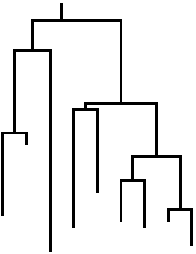
\includegraphics[width=37.7\unitlength]{phylo-b}}
\cell{6.5}{9}{b}{1}
\cell{11}{23.5}{b}{2}
\cell{15.6}{3}{b}{3}
\cell{20.1}{7.5}{b}{4}
\cell{24.7}{14}{b}{5}
\cell{29.1}{8.5}{b}{6}
\cell{33.7}{7}{b}{7}
\cell{38.2}{8.5}{b}{8}
\cell{42.8}{3.5}{b}{9}
\cell{24.6}{-2}{b}{(b)}
\end{picture}%
\hspace*{7\unitlength}%
\begin{picture}(24,57)(0,3)
\cell{13.5}{31.5}{c}{\includegraphics[width=21\unitlength]{phylo-c}}
\cell{4}{12.5}{c}{1}
\cell{13.5}{14}{c}{2}
\cell{23}{17.5}{c}{3}
\cell{14.5}{43}{c}{\normalsize$b_1$}
\cell{6}{34}{c}{\normalsize$b_2$}
\cell{1.5}{22}{c}{\normalsize$b_3$}
\cell{16.5}{23}{c}{\normalsize$b_4$}
\cell{20.5}{28}{c}{\normalsize$b_5$}
\cell{13.5}{3}{b}{(c)}
\end{picture}%
\caption{Simple examples of phylogenetic trees, with present-day species
  labelled as $1, 2, \ldots$\:\  Tree~\hardref{(a)} is ultrametric, but
  trees~\hardref{(b)} and~\hardref{(c)} are not.  Tree~\hardref{(c)} has
  five branches, shown as thick lines and labelled as $b_1, \ldots, b_5$.}  
\lbl{fig:phylo-trees}
\end{figure}
% 
The vertical axis indicates time, or some proxy for time; the horizontal
distances in the trees mean nothing.
Figure~\ref{fig:phylo-trees}\hardref{(a)} shows nine species descended from
a single species.  In that example, the tree is
\demph{ultrametric}\index{ultrametric!tree}, meaning that the tips of the
tree (the present-day species) are all at the same height.

Evolutionary history is often inferred from genetic data,
with the number of genetic mutations used as a means of estimating time.
Because the rate of genetic mutation is not constant (and for other
reasons), the trees produced in this way are generally not ultrametric.
Figure~\ref{fig:phylo-trees}\hardref{(b)} shows an example.  

From a phylogenetic tree, we can extract the following information:
% 
\begin{itemize}
\item 
the set of present-day species, which we label as $1, \ldots, S$;

\item
the set $B$ of branches;

\item
the binary relation $\descd$\ntn{descd}, where for a present-day species $r$
and a branch $b$, we write $r \descd b$ if $r$ is descended from $b$;

\item
the length $L(b) \geq 0$ of each branch $b$.
\end{itemize}
% 
These four pieces of information are the only aspects of a tree that we
will need for the present purposes.  For instance, the tree of
Figure~\ref{fig:phylo-trees}\hardref{(c)} has $S = 3$, $B = \{b_1, b_2,
b_3, b_4, b_5\}$, and
% 
\begin{align*}
&1 \descd b_1, \ 1 \descd b_2, \ 1 \descd b_3, \\
&2 \descd b_1, \ 2 \descd b_2, \ 2 \descd b_4, \\
&3 \descd b_1, \ 3 \descd b_5.
\end{align*}
% 
We do not require that the present-day species are all descended from a
common ancestor within the time span considered; that is, the `tree' may
actually consist of several disjoint trees (a
forest,\index{forest!mathematical} in mathematical terminology).

We will consider measures of community diversity based on two factors: a
phylogenetic tree for the species, and their present-day relative abundance
distribution $(\pi_1, \ldots, \pi_S)$.  To do this, we introduce some
notation.

For each branch $b$, write
% 
\begin{equation}
\lbl{eq:ccj-abun}
\pi(b) = \sum_{r \csuch r \descd b} \pi_r,
\end{equation}
% 
which is the total relative abundance of present-day species descended from
branch $b$.  So if the tree is ultrametric then whenever we draw a
horizontal line across the tree (representing a particular point $t$ in
evolutionary time), the sum of $\pi(b)$ over all branches $b$ intersecting
that line is $1$.  For any given point in evolutionary time, we therefore
have a probability distribution on the set of species present then,
although as Chao%
%
\index{Chao, Anne} 
% 
et al.\ warn, `These abundances [$\pi(b)$] are not estimates of the actual
abundances of these ancestral species at time $t$, but rather measures of
their importance for the present-day assemblage' (\cite{CCJ},
Section~4(a)).

For each present-day species $r \in \{1, \ldots, S\}$, write
\[
L_r = \sum_{b \csuch r \descd b} L(b).
\]
This is the length of the lineage of species $r$ within the tree.  For the
tree to be ultrametric means that $L_1 = \cdots = L_S$.  Whether or not it
is ultrametric, we can define the average lineage length $\ovln{L}$ by any
of three equivalent formulas:
\[
\ovln{L}
=
\sum_r \pi_r L_r
=
\sum_{r, b \csuch r \descd b} \pi_r L(b)
=
\sum_b \pi(b) L(b).
\]
Hence $\ovln{L}$ is the expected lineage length of an individual chosen at
random from the present-day community.  

Chao, Chiu and Jost defined a phylogenetic diversity measure as follows.
For each time point $t$ in the period under consideration, they took the
abundance distribution described below equation~\eqref{eq:ccj-abun}.  They
then took its Hill number of order $q$, and formed the average of these
Hill numbers over all times $t$.  After some simplification, the result is
the diversity measure
\[
\CCJ{q}
=
\Biggl( \sum_b \frac{L(b)}{\ovln{L}} \pi(b)^q \Biggr)^{1/(1 - q)}
\]
for $1 \neq q \in [0, \infty)$, and 
\[
\CCJ{1}
=
\prod_b \pi(b)^{-{\textstyle\frac{L(b)}{\ovln{L}}} \pi(b)}.
\]
(Their derivation is on its surest footing when the tree is ultrametric.
Discussion of what can go wrong otherwise is in the supplement to
Chao et al.~\cite{CCJ} and in Example~A20 of the appendix to
Leinster and Cobbold~\cite{MDISS}.)  For example, the case $q = 0$ is
simply
\[
\CCJ{0} = \frac{1}{\ovln{L}} \sum_b L(b).
\]
Up to a factor of $\ovln{L}$, this is the total length of all the branches
in the tree, which is known as \demph{Faith's phylogenetic
  diversity}~\cite{Fait}.%
%
\index{Faith's phylogenetic diversity}

We now show that Chao, Chiu and Jost's measure $\CCJ{q}$ is a simple
instance of the value measure $\sigma_q$.  For this, we consider the
phylogenetic tree as our whole and the branches as its parts.
The value of a branch $b$ is defined as 
\[
v(b) = \frac{L(b)}{\ovln{L}},
\]
the proportion of evolutionary time over which the branch extends.  It is
purely a measure of the branch's historical duration, and is independent of
the abundances of present-day species.  We define the relative size $p(b)$
of the branch to be
\[
p(b) = \frac{\pi(b) L(b)}{\ovln{L}}.
\]
In other words, $p(b)$ is the product of $\pi(b)$, the proportion of
present-day individuals descended from branch $b$, and $L(b)/\ovln{L}$, the
relative length of the branch.  Then $\sum_b p(b) = 1$.

With these definitions, the value $\sigma_q(\p, \vc{v})$ of the community
is
% 
\begin{align*}
\sigma_q(\p, \vc{v})    &
=
\Biggl( \sum_b p(b)^q v(b)^{1 - q} \Biggr)^{1/(1 - q)}  \\
&
=
\Biggl( 
\sum_b 
\frac{\pi(b)^q L(b)^q}{\ovln{L}^q}
\frac{L(b)^{1 - q}}{\ovln{L}^{1 - q}}
\Biggr)^{1/(1 - q)}     \\
&
=
\Biggl( 
\sum_b 
\frac{L(b)}{\ovln{L}} \pi(b)^q
\Biggr)^{1/(1 - q)}      \\
&
=
\CCJ{q}
\end{align*}
% 
($q \neq 1, \infty$).  Similarly, $\sigma_1(\p, \vc{v}) = \CCJ{1}$.

The community value $\sigma_q(\p, \vc{v}) = \CCJ{q}$ is unitless, since the
individual branch values $v(b) = L(b)/\ovln{L}$ are unitless.  We could
alternatively put $v(b) = L(b)$, which might be measured in years or number
of mutations.  Then $\sigma_q(\p, \vc{v})$ would be measured in the same
units, and $\sigma_0(\p, \vc{v})$ would be exactly Faith's
phylogenetic diversity, without the factor of $1/\ovln{L}$.
\end{example}

In summary, the value measures $\sigma_q$ unify not only the Hill numbers
$D_q$, the similarity-sensitive diversity measures $D_q^Z$, and the
diversity of a community divided into completely dissimilar subcommunities
(Example~\ref{eg:value-ch}), but also some known measures of phylogenetic
diversity.

One could also assign a value to each species in a more literal,
utilitarian\index{utilitarianism} sense (perhaps
monetary).%
%
\index{economics}%
\index{value!monetary}%
\index{value!medicinal}
% 
Solow%
%
\index{Solow, Andrew} 
%
and
Polasky%
%
\index{Polasky, Stephen} 
% 
noted that `one justification for species
conservation\index{conservation} is that some species may provide a future
medical benefit' (\cite{SoPo}, p.~98), and analysed diversity from that
viewpoint.  This line of enquiry is worthwhile not only for the evident
scientific reasons, but also because it is how Solow and Polasky arrived at
the mathematically profound invariant now called magnitude (as related on
p.~\pageref{p:sp-mag}).  But we will not pursue it, instead making a
connection between value measures and established quantities in information
theory.


\section{Value and relative entropy}
\lbl{sec:value-rel}
\index{value!relative entropy@and relative entropy}
\index{relative entropy!value@and value}


The value measure $\sigma_q$ is a simple transformation of a classical
object of study, the R\'enyi relative entropy or R\'enyi divergence
(R\'enyi~\cite{Reny}, Section~3).  In this short section, we describe the
relationship between value, relative entropy, and some of the other
quantities that we have considered.  This provides useful context, although
nothing here is logically necessary for anything that follows.

For $q \in [-\infty, \infty]$ and probability
distributions $\p, \vc{r} \in \Delta_n$, the \demph{R\'enyi entropy of
  order $q$ of $\p$ relative to $\vc{r}$}%
%
\index{Renyi relative entropy@R\'enyi relative entropy}%
\index{order!Renyi relative entropy@of R\'enyi relative entropy}
% 
is defined as 
\[
\hrelent{q}{\p}{\vc{r}}
=
\frac{1}{q - 1} \log \sum_{i \in \supp(\p)} p_i^q r_i^{1 - q}
\ntn{hrelent}
\]
when $q \neq 1, \pm \infty$, and in the exceptional cases by
% 
\begin{align*}
\hrelent{-\infty}{\p}{\vc{r}}   &
=
\log\min_{i \in \supp(\p)} \frac{p_i}{r_i},    \\
\hrelent{1}{\p}{\vc{r}} &
=
\sum_{i \in \supp(\p)} p_i \log \frac{p_i}{r_i}
=
\relent{\p}{\vc{r}},    \\
\hrelent{\infty}{\p}{\vc{r}}    &
=
\log\max_{i \in \supp(\p)} \frac{p_i}{r_i}.
\end{align*}
% 
In all cases, 
\[
\hrelent{q}{\p}{\vc{r}} 
= 
\log M_{q - 1}(\vc{p}, \vc{p}/\vc{r})
=
-\log M_{1 - q}(\vc{p}, \vc{r}/\vc{p})
\]
(by the duality equation~\eqref{eq:mn-duality},
p.~\pageref{eq:mn-duality}), giving
% 
\begin{equation}
\lbl{eq:val-rel-ent}
\hrelent{q}{\p}{\vc{r}}
=
-\log \sigma_q(\p, \vc{r}).
\end{equation}
% 
R\'enyi relative entropy can take the value $\infty$.  But as for classical
relative entropy ($q = 1$, p.~\pageref{p:An}), it is convenient to restrict
to pairs $(\vc{p}, \vc{r})$ such that $p_i = 0$ whenever $r_i = 0$; then
$\hrelent{q}{\vc{p}}{\vc{r}} < \infty$ for all $q$.

The R\'enyi relative entropies share with the classical version the basic
property that $\hrelent{q}{\p}{\p} = 0$ for all distributions $\p$.
When $q > 0$, they also share its positive definiteness property,
stated in the classical case as Lemma~\ref{lemma:rel-ent-pos-def}: 

\begin{lemma}
For all $q > 0$ and $\vc{p}, \vc{r} \in \Delta_n$,
\[
\hrelent{q}{\p}{\vc{r}} \geq 0,
\]
with equality if and only if $\vc{p} = \vc{r}$.
\end{lemma}

\begin{proof}
This follows from equation~\eqref{eq:val-rel-ent} and
Lemma~\ref{lemma:sigma-sum-ineq}, since $\sum_{i = 1}^n r_i = 1$.
\end{proof}

In the definition above of R\'enyi relative entropy, both arguments were
required to be probability distributions, whereas the second argument
$\vc{v}$ of the value measure $\sigma_q$ can be any vector of nonnegative
reals.  In fact, when R\'enyi introduced his relative entropies, he allowed
$\p$ and $\vc{r}$ to be `generalized%
%
\index{generalized probability distribution}%
\index{probability distribution!generalized}
%
probability distributions' (vectors of nonnegative reals summing to
\emph{at most} $1$), and he inserted a normalizing factor of $\sum p_i$
accordingly (Section~3 of~\cite{Reny}).  But we will consider relative
entropy only for pairs of genuine probability distributions.

Just as R\'enyi relative entropy of order $q$ is closely related to the
value measure $\sigma_q$, so too is $q$-logarithmic relative entropy
\[
\srelent{q}{\p}{\vc{r}}
=
- \sum_{i \in \supp(\p)} p_i \ln_q \frac{r_i}{p_i}
\]
(Definition~\ref{defn:q-rel-ent}).  The formula for $q$-logarithmic
relative entropy in terms of value is the same as the
formula~\eqref{eq:val-rel-ent} for R\'enyi relative entropy in terms of
value, but with the logarithm replaced by the $q$-logarithm:
\[
\srelent{q}{\p}{\vc{r}}
=
- \ln_q \sigma_q(\p, \vc{r})
\]
($-\infty < q < \infty$).  To prove this, we use
Lemma~\ref{lemma:q-log-mean}: 
% 
\begin{align*}
\srelent{q}{\p}{\vc{r}}
&
=
- M_1 \bigl(\p, \ln_q(\vc{r}/\p) \bigr) \\
&
=
- \ln_q M_{1 - q} (\p, \vc{r}/\p) \\
&
=
- \ln_q \sigma_q(\p, \vc{r}).     
\end{align*}
% 
Hence $\sigma_q(-,-)$, $\hrelent{q}{-}{-}$ and $\srelent{q}{-}{-}$ are
all simple transformations of one another.

R\'enyi relative entropy shares with ordinary relative entropy the
property that
\[
\hrelent{q}{\p}{\vc{u}_n}
% =
% \log n - H_q(\p)
=
H_q(\vc{u}_n) - H_q(\p)
\]
($q \in [-\infty, \infty]$, $\p \in \Delta_n$).  In this respect, R\'enyi
relative entropy has slightly more%
%
\index{Renyi relative entropy@R\'enyi relative entropy!q-logarithmic@and $q$-logarithmic relative entropy}%
\index{q-logarithmic relative entropy@$q$-logarithmic relative entropy!Renyi@and R\'enyi relative entropy}
%
convenient algebraic properties than
$q$-logarithmic relative entropy: compare the formula for
$\srelent{q}{\p}{\vc{u}_n}$ in Remark~\ref{rmk:q-rel-ent-param}.

\begin{remark}
\lbl{rmk:gen-def-rel}
In Remark~\ref{rmk:gen-def}, we observed that for any differentiable
function $\lambda\from (0, \infty) \to \R$ satisfying $\lambda(1) = 0$ and
$\lambda'(1) = 1$, the formula
\[
\frac{1}{1 - q} \, 
\lambda\,
\Biggl( \sum_{i \in \supp(\p)} p_i^q \Biggr)
\]
defines a one-parameter family of deformations of Shannon entropy, in the
sense that it converges to $H(\p)$ as $q \to 1$.  A similar statement holds
for relative entropy: for any such function $\lambda$, the generalized
relative entropy
\[
\frac{1}{q - 1} \,
\lambda\,
\Biggl( \sum_{i \in \supp(\p)} p_i^q r_i^{1 - q} \Biggr)
\]
converges to the ordinary relative entropy $\relent{\p}{\vc{r}}$ as $q \to
1$.  Taking $\lambda = \log$ gives R\'enyi relative entropy, and taking
$\lambda(x) = x - 1$ gives $q$-logarithmic relative entropy.
\end{remark}

\begin{remarks}
\lbl{rmks:fisher-def}
Here we relate the deformed relative entropies to the
Fisher%
%
\index{Fisher, Ronald!metric} 
% 
metric on probability distributions.
% 
\begin{enumerate}
\item
\lbl{rmk:fisher-def-gods-joke}
% 
In Section~\ref{sec:rel-misc}, we showed that although the square root of
ordinary relative entropy is not a distance function on the open simplex
$\Delta_n^\circ$ (that is, not a metric in the sense of metric spaces), it
is an \emph{infinitesimal} metric in the Riemannian sense.  As we saw, it
is proportional to the Fisher metric, which itself is proportional to the
standard Riemannian metric on the positive orthant of the unit sphere,
transferred to $\Delta_n^\circ$ via the bijection $\p \leftrightarrow
\sqrt{\p}$.

It is natural to ask what happens if we apply the same procedure to the
R\'enyi relative entropy of order $q$, or the $q$-logarithmic relative
entropy, for some $q \neq 1$.  Do we obtain some new, deformed, Fisher-like
metric on $\Delta_n^\circ$?

The answer turns out to be no.  Using $\hrelent{q}{-}{-}$ or
$\srelent{q}{-}{-}$ instead of the ordinary relative entropy
$\relent{-}{-}$ simply multiplies the induced metric on $\Delta_n^\circ$ by
a constant factor of $q$.  More generally, the same is true of any family
of deformations of relative entropy of the type constructed in
Remark~\ref{rmk:gen-def-rel}. 
(We omit the proof, but it is similar to the argument for ordinary relative
entropy; compare also Section~2.7 of Ay, Jost, L{\^e} and
Schwachh{\"o}fer~\cite{AJLS} and Chapter~3 of Amari~\cite{AmarIGA}.)
It follows that the $q$-analogues of
Fisher%
%
\index{Fisher, Ronald!distance}  
%
distance and Fisher%
%
\index{Fisher, Ronald!information}
%
information (defined as in equation~\eqref{eq:fisher-info}) are
proportional to the classical Fisher distance and information, and that the
$q$-analogue of the Jeffreys%
%
\index{Jeffreys, Harold!prior}
% 
prior is exactly equal to the classical notion.

The moral is that the Fisher metric on probability distributions is a very
stable, canonical concept.  However we may choose to deform relative
entropy, the induced metric is always essentially the same.

\item
The parameter value $q = 1/2$ plays a special role.  The R\'enyi%
%
\index{Renyi relative entropy@R\'enyi relative entropy!order 1@of order $1/2$}
% 
and $q$-logarithmic%
%
\index{q-logarithmic relative entropy@$q$-logarithmic relative entropy!order 1@of order $1/2$}
% 
relative entropies of order $1/2$ are
\[
\hrelent{1/2}{\p}{\vc{r}} = -2 \log \sum \sqrt{p_i r_i},
\qquad
\srelent{1/2}{\p}{\vc{r}} = 2 \biggl( 1 - \sum \sqrt{p_i r_i} \biggr).
\]
Both are symmetric in $\p$ and $\vc{r}$ (and $q = 1/2$ is the only
parameter value with this property).  In fact, both are
increasing, invertible transformations of the Fisher%
%
\index{Fisher, Ronald!distance}
% 
distance
\[
d_\fishsym(\p, \vc{r}) 
= 
2 \cos^{-1} \biggl( \sum \sqrt{p_i r_i} \biggr).
\]
Thus, the R\'enyi relative entropy of order $1/2$ of a pair of
distributions determines the Fisher distance between them.  Similarly,
knowing either the $(1/2)$-logarithmic entropy of $(\p, \vc{r})$ or the
value of order $1/2$,
\[
\sigma_{1/2}(\p, \vc{r}) = \biggl( \sum \sqrt{p_i r_i} \biggr)^2,
\]
determines the Fisher distance between $\p$ and $\vc{r}$.
\end{enumerate}
\end{remarks}


\section{Characterization of value}
\lbl{sec:value-char}
\index{value measure!characterization of}

 
Here we show that the only value measures with reasonable properties are
those of the form $\sigma_q$ for some $q \in [-\infty, \infty]$.  

We defined the value measure $\sigma_q$ on the nonnegative half-line $[0,
  \infty)$, but it restricts to a sequence of functions
\[
\bigl( 
\sigma_q \from \Delta_n \times (0, \infty)^n \to (0, \infty) 
\bigr)_{n \geq 1}
\]
on the strictly positive reals. It is this family $(\sigma_q)_{q \in
  [-\infty, \infty]}$ that we will characterize.  A similar theorem on $[0,
  \infty)$ can be proved, at the cost of an extra hypothesis
  (Remark~\ref{rmk:val-char-nonneg}), but we will focus on strictly
  positive values.
% 
Thus, we will identify a list of conditions on a sequence of functions
% 
\begin{equation}
\lbl{eq:typ-val}
\bigl( 
\sigma \from \Delta_n \times (0, \infty)^n \to (0, \infty) 
\bigr)_{n \geq 1}
\end{equation}
% 
that are satisfied by $\sigma_q$ for each $q \in [-\infty, \infty]$, but
not by any other $\sigma$.

We begin by describing those conditions.  

Recall that a weighted mean $M$ on $(0, \infty)$ is a sequence of functions
of the same type as a value measure on $(0, \infty)$:
\[
\bigl( 
M \from \Delta_n \times (0, \infty)^n \to (0, \infty) 
\bigr)_{n \geq 1}.
\]
Although the classes of reasonable means and reasonable value measures
are intended to be disjoint (Remark~\ref{rmk:vals-mns}), some of the
properties that one expects of a mean can also be expected of a value
measure.  We therefore reuse some of the terminology defined previously
for weighted means, and summarized in Appendix~\ref{app:condns}.  

In what follows, let $\sigma$ denote a sequence of
functions as in~\eqref{eq:typ-val}.
% \[
% \bigl( 
% \sigma \from \Delta_n \times (0, \infty)^n \to (0, \infty) 
% \bigr)_{n \geq 1}.
% \]
Then $\sigma$ may or may not have the following properties, all defined
previously in the context of weighted means.

\begin{description}
\item[Symmetry.]%
\index{symmetric!value measure}%
\index{value measure!symmetric}
% 
For $\sigma$ to be symmetric
(Definition~\ref{defn:pwr-mn-elem}\bref{part:pme-sym}) means that the value
of the whole is independent of the order in which the parts are listed.

\item[Absence-invariance.]%
\index{absence-invariance!value measure@of value measure}%
\index{value measure!absence-invariant}
% 
For $\sigma$ to be absence-invariant
  (Definition~\ref{defn:pwr-mn-elem}\bref{part:pme-abs}) means that a part
  that is absent ($p_i = 0$) makes no contribution to the value of the
  whole, and might as well be ignored.

\item[Increasing.]%
\index{increasing!value measure}%
\index{value measure!increasing}
% 
For $\sigma$ to be increasing (Definition~\ref{defn:w-isi}) means that the
parts make a positive (or at least, nonnegative) contribution to the
whole: if the value of one part increases and the rest stay the same, this
does not cause the value of the whole to become smaller.

\item[Homogeneity.]%
\index{homogeneous!value measure}%
\index{value measure!homogeneous}
% 
Homogeneity of $\sigma$ (Definition~\ref{defn:w-mn-hgs}) means that the
value of the whole and the values of the parts are measured in the same
units.  For instance, if the value of each part is measured in kilograms
then so is the value of the whole.  Converting to grams multiplies both by
$1000$.

\item[Chain rule.]%
\index{chain rule!value measures@for value measures}%
\index{value measure!chain rule for}
% 
The chain rule for $\sigma$ (Definition~\ref{defn:mns-chn}) is the most
complicated of the properties that we will need, but it is logically
fundamental.  It states that
% 
\begin{align}
\nonumber
&
\sigma\bigl( \vc{w} \of (\p^1, \ldots, \p^n),
\vc{v}^1 \oplus\cdots\oplus \vc{v}^n \bigr)
\\
\lbl{eq:val-ch}
=\ 
&
\sigma\Bigl(
\vc{w}, 
\bigl(
\sigma(\p^1, \vc{v}^1), \ldots, \sigma(\p^n, \vc{v}^n) 
\bigr)
\Bigr)  
\end{align}
% 
for all $n, k_1, \ldots, k_n \geq 1$, $\vc{w} \in \Delta_n$, $\p^i \in
\Delta_{k_i}$, and $\vc{v}^i \in (0, \infty)^{k_i}$.  

\begin{figure}
\centering
\lengths
\begin{picture}(120,44)
\cell{60}{22}{c}{\includegraphics[height=44\unitlength]{value_chainm}}
\cell{2}{22}{c}{\large$w_1$}
\cell{118}{30}{c}{\large$w_2$}
\cell{118}{9}{c}{\large$w_3$}
% 
\cell{18}{35}{c}{$p^1_1$}
\valput{24}{32}{$v^1_1$}
\cell{55}{30}{c}{$p^1_2$}
\valput{61}{27}{$v^1_2$}
\cell{18}{10}{c}{$p^1_3$}
\valput{24}{7}{$v^1_3$}
\cell{43}{11}{c}{$p^1_4$}
\valput{49}{8}{$v^1_4$}
% 
\cell{85}{31}{c}{$p^2_1$}
\valput{91}{28}{$v^2_1$}
\cell{102}{31}{c}{$p^2_2$}
\valput{108}{28}{$v^2_2$}
% 
\cell{75.5}{10.5}{c}{$p^3_1$}
\valput{75.5}{4.5}{$v^3_1$}
\cell{83.5}{10.5}{c}{$p^3_2$}
\valput{83.5}{4.5}{$v^3_2$}
\cell{91.5}{10.5}{c}{$p^3_3$}
\valput{91.5}{4.5}{$v^3_3$}
\cell{99}{10.5}{c}{$p^3_4$}
\valput{99}{4.5}{$v^3_4$}
\cell{108}{10.5}{c}{$p^3_5$}
\valput{108}{4.5}{$v^3_5$}
\end{picture}
\caption{The chain rule for value measures, as in
  equation~\eqref{eq:val-ch}.  Here, the whole is divided into $n = 3$
  parts, the first part is divided into $k_1 = 4$ subparts, the second
  into $k_2 = 2$ subparts, and the third into $k_3 = 5$ subparts.}
\lbl{fig:val-ch}  
\end{figure}

This is a recursivity property (Figure~\ref{fig:val-ch}).  It means that
our method $\sigma$ of aggregating value behaves consistently when the
whole is divided into parts which are further divided into subparts.

Suppose, for example, that we are performing some evaluation of the
whole planetary landmass, and that we have already assigned a value to each
country.  We could first use $\sigma$ to compute the value of each
continent, then use $\sigma$ again on those continental values to compute
the global value.  This is the right-hand side of
equation~\eqref{eq:val-ch}, if $v^i_j$ denotes the value of the $j$th
country on the $i$th continent, $\p^i$ is the relative size distribution of
the countries on the $i$th continent, and $\vc{w}$ is the relative size
distribution of the continents.  Alternatively, we could
ignore the intermediate level of continents and use $\sigma$ to compute the
global value directly from the country values.  This gives the left-hand
side of equation~\eqref{eq:val-ch}.  The two methods for computing the
global value should give the same result, and the chain rule states that
they do.
\end{description}

We make two further definitions for value measures $\sigma$ on $(0,
\infty)$.

\begin{defn}
\lbl{defn:val-cipp}
$\sigma$ is \demph{continuous%
%
\index{continuous!positive probabilities@in positive probabilities} 
% 
in positive probabilities} if for each $n \geq 1$ and $\vc{v} \in (0,
\infty)^n$, the function
\[
\begin{array}{cccc}
\sigma(-, \vc{v}):      &\Delta_n^\circ  &\to            &(0, \infty)    \\
                        &\p              &\mapsto        &\sigma(\p, \vc{v})
\end{array}
\]
on the open simplex is continuous.
\end{defn}

This condition only involves continuity in the \emph{sizes} of the parts
present, not their values.  The restriction to the interior of the simplex
means that we do not forbid value measures that make a sharp distinction
between presence and absence.

\begin{defn}
\lbl{defn:val-eff}
$\sigma$ is an \demph{effective%
%
\index{effective number}
%
number} if 
\[
\sigma\bigl( \vc{u}_n, (1, \ldots, 1) \bigr) = n
\]
for all $n \geq 1$.
\end{defn}

Assuming homogeneity, the effective number property is equivalent to 
% 
\begin{equation}
\lbl{eq:val-eff-rep}
\sigma\bigl(\vc{u}_n, (v, \ldots, v)\bigr) = nv
\end{equation}
% 
for all $n \geq 1$ and $v \in (0, \infty)$.  That is, if we put together
$n$ parts of equal size and equal value, $v$, the result has value $nv$.  

\begin{remark}
\lbl{rmk:val-undef}
Let $\sigma$ be an absence-invariant value measure.  Then $\sigma(\p,
\vc{v})$ is independent of $v_i$ for $i \not\in \supp(\p)$.  Indeed,
writing $\supp(\p) = \{i_1, \ldots, i_k\}$ with $i_1 < \cdots < i_k$,
absence-invariance implies that
% 
\begin{equation}
\lbl{eq:val-supp}
\sigma(\p, \vc{v})
=
\sigma\bigl( (p_{i_1}, \ldots, p_{i_k}), (v_{i_1}, \ldots, v_{i_k}) \bigr).
\end{equation}
% 
So we can consistently extend%
%
\index{value!undefined}%
\index{undefined arguments} 
% 
the definition of $\sigma(\p, \vc{v})$ to pairs $(\p, \vc{v})$ where $v_i$
need not be within the permissible range $(0, \infty)$, or even defined at
all, when $i \not\in \supp(\p)$.  In that case, we define $\sigma(\p,
\vc{v})$ to be the right-hand side of equation~\eqref{eq:val-supp}.  This
convention is exactly analogous to the convention for means introduced in
Remark~\ref{rmk:defined-even-if-not}, and to the usual convention for
integrals of functions undefined on a set of measure zero.
\end{remark}

We now prove that the properties listed above uniquely characterize the
family of value measures $(\sigma_q)$.

\begin{thm}
\lbl{thm:val-char}
\index{value measure!characterization of}
% 
Let $\bigl( \sigma \from \Delta_n \times (0, \infty)^n \to (0, \infty)
\bigr)_{n \geq 1}$ be a sequence of functions.  The following are
equivalent: 
% 
\begin{enumerate}
\item 
\lbl{part:val-char-condns}
$\sigma$ is symmetric, absence-invariant, increasing, homogeneous,
continuous in positive probabilities and an effective number, and satisfies
the chain rule;

\item
\lbl{part:val-char-form}
$\sigma = \sigma_q$ for some $q \in [-\infty, \infty]$. 
\end{enumerate}
\end{thm}

\begin{proof}
To prove that~\bref{part:val-char-form}
implies~\bref{part:val-char-condns}, let $q \in [-\infty, \infty]$.  
That $\sigma_q$ is symmetric, absence-invariant, increasing, homogeneous, and
continuous in positive probabilities follows from
the definition
\[
\sigma_q(\p, \vc{v}) = M_{1 - q}(\p, \vc{v}/\p)
\]
of $\sigma_q$ and the corresponding properties of $M_{1 - q}$
(Lemmas~\ref{lemma:pwr-mns-elem}, \ref{lemma:pwr-mns-inc},
\ref{lemma:pwr-mns-hgs} and
\ref{lemma:pwr-mns-cts-px}\bref{part:pwr-mns-cts-px-1}).  That $\sigma_q$
is an effective number follows from the consistency of $M_{1 - q}$, and the
chain rule for $\sigma_q$ follows from the chain rule for $M_{1 - q}$
(Proposition~\ref{propn:pwr-mns-chn}).

Conversely, assume that $\sigma$ satisfies the conditions
in~\bref{part:val-char-condns}.  Define a sequence of functions
\[
\bigl( 
M \from \Delta_n \times (0, \infty)^n \to (0, \infty) 
\bigr)_{n \geq 1}
\]
by 
\[
M(\p, \vc{x}) = \sigma(\p, \p\vc{x})
\]
($\p \in \Delta_n$, $\vc{x} \in (0, \infty)^n$).  Although it may be that
$(\p\vc{x})_i = 0$ for some $i$, in which case $\sigma(\p, \p\vc{x})$ is
strictly speaking undefined, this can only happen when $p_i = 0$; hence
$\sigma(\p, \p\vc{x})$ can be interpreted according to the convention of
Remark~\ref{rmk:val-undef}.

We will prove that $M$ is a power mean.  We do this by showing that $M$
satisfies the hypotheses of Theorem~\ref{thm:w-inc}: $M$ is symmetric,
absence-invariant, increasing, homogeneous, modular, and consistent.  The
first four follow from the corresponding properties of $\sigma$.
It remains to prove that $M$ is modular and consistent.

For modularity, let $\vc{w} \in \Delta_n$, $\p^i \in \Delta_{k_i}$, and
$\vc{x}^i \in (0, \infty)^{k_i}$.  Using the chain rule and
homogeneity properties of $\sigma$, we find that
% 
\begin{align*}
&
M\bigl( 
\vc{w} \of (\p^1, \ldots, \p^n), \vc{x}^1 \oplus\cdots\oplus \vc{x}^n
\bigr)  \\
&
=
\sigma\bigl(
\vc{w} \of (\p^1, \ldots, \p^n), 
w_1 \p^1 \vc{x}^1 \oplus\cdots\oplus w_n \p^n \vc{x}^n
\bigr)  \\
&
=
\sigma\Bigl(
\vc{w}, \bigl(
\sigma\bigl(\p^1, w_1 \p^1 \vc{x}^1\bigr), 
\ldots, 
\sigma\bigl(\p^n, w_n \p^n \vc{x}^n\bigr)
\bigr)
\Bigr)  \\
&
=
\sigma\Bigl(
\vc{w}, \bigl(
w_1 M(\p^1, \vc{x}^1), \ldots, w_n M(\p^n, \vc{x}^n)
\bigr)
\Bigr)  \\
&
=
M\Bigl(
\vc{w}, \bigl(
M(\p^1, \vc{x}^1), \ldots, M(\p^n, \vc{x}^n)
\bigr)
\Bigr).
\end{align*}
% 
Hence $M$ satisfies the chain rule, and is therefore modular.

Proving that $M$ is consistent is equivalent, by homogeneity, to showing that
\[
\sigma(\p, \p) = 1
\]
for all $n \geq 1$ and $\p \in \Delta_n$.  We do this in three steps.

First suppose that the coordinates of $\p$ are positive and rational, so
that $\p = (k_1/k, \ldots, k_n/k)$ for some positive integers $k_i$ summing
to $k$.  Then
\[
\vc{u}_k = \p \of (\vc{u}_{k_1}, \ldots, \vc{u}_{k_n}),
\]
so by the chain rule for $\sigma$,
\[
\sigma(\vc{u}_k, k \mc 1)
=
\sigma\Bigl(
\p, \bigl(
\sigma(\vc{u}_{k_1}, k_1 \mc 1), \ldots, \sigma(\vc{u}_{k_n}, k_n \mc 1)
\bigr)
\Bigr).
\]
By the effective number property of $\sigma$, this means that
\[
k = \sigma\bigl( \p, (k_1, \ldots, k_n)\bigr).
\]
Dividing through by $k$ and using the homogeneity of $\sigma$ gives $1 =
\sigma(\p, \p)$, as required.

For the second step, let $\p$ be any point in $\Delta_n^\circ$.  Let
$\epsln > 0$.  Since $\sigma$ is continuous in positive probabilities,
there is some $\delta > 0$ such that for $\vc{r} \in \Delta_n^\circ$,
% 
\begin{equation}
\lbl{eq:vc-imp}
\|\p - \vc{r}\| < \delta
\implies
\mg{\sigma(\p, \p) - \sigma(\vc{r}, \p)} < \epsln/2,
\end{equation}
% 
where $\|\cdot\|$ denotes Euclidean length.  We can choose $\vc{r} \in
\Delta_n^\circ$ with rational coordinates such that
\[
\|\p - \vc{r}\| < \delta,
\quad
\max_i \frac{p_i}{r_i} \leq 1 + \frac{\epsln}{2},
\quad
\min_i \frac{p_i}{r_i} \geq 1 - \frac{\epsln}{2}.
\]
Since $\sigma$ is increasing and homogeneous,
\[
\sigma(\vc{r}, \p) 
\leq
\sigma\biggl(\vc{r}, \biggl(\max_i \frac{p_i}{r_i}\biggr) \vc{r}\biggr)
=
\biggl(\max_i \frac{p_i}{r_i}\biggr) \sigma(\vc{r}, \vc{r}),
\]
which by the first step gives
\[
\sigma(\vc{r}, \vc{p}) \leq \max_i \frac{p_i}{r_i} 
\leq 1 + \frac{\epsln}{2}.
\]
Similarly, $\sigma(\vc{r}, \p) \geq 1 - \epsln/2$, so
\[
\mg{\sigma(\vc{r}, \p) - 1} \leq \epsln/2.
\]
This, together with~\eqref{eq:vc-imp} and the triangle inequality, implies
that $\mg{\sigma(\p, \p) - 1} < \epsln$.  But $\epsln$ was arbitrary, so
$\sigma(\p, \p) = 1$.

Third and finally, take any $\p \in \Delta_n$.  Write $\supp(\p) = \{i_1,
\ldots, i_k\}$ with $i_1 < \cdots < i_k$, and write $\vc{r} =
(p_{i_1}, \ldots, p_{i_k}) \in \Delta_k^\circ$.  Then 
\[
\sigma(\p, \p) = \sigma(\vc{r}, \vc{r}) = 1,
\]
where the first equality holds for the reasons given in
Remark~\ref{rmk:val-undef}, and the second follows from the second step
above. 

This completes the proof that $M$ is consistent.  We have now shown
that $M$ satisfies the hypotheses of Theorem~\ref{thm:w-inc}.  By that
theorem, $M = M_{1 - q}$ for some $q \in [-\infty, \infty]$.  It follows
that
\[
\sigma(\p, \vc{v})
=
% M(\p, \vc{v}/\p)
% =
M_{1 - q}(\p, \vc{v}/\p)
=
\sigma_q(\p, \vc{v})
\]
for all $n \geq 1$, $\p \in \Delta_n$, and $\vc{v} \in (0, \infty)^n$.
\end{proof}


\begin{remark}
\lbl{rmk:val-char-nonneg} 
A similar characterization theorem can be proved for values in $[0,
  \infty)$ instead of $(0, \infty)$, using Theorem~\ref{thm:w-cts-inc} on
  means on $[0, \infty)$.  In this case, we have to strengthen the
    continuity requirement, also asking that $\sigma(\p, \vc{v})$ is
    continuous in $\vc{v}$ for each fixed $\p$. 
\end{remark}

Theorem~\ref{thm:val-char} can be translated into a characterization
theorem for either the R\'enyi relative entropies or the $q$-logarithmic
relative entropies, using the observations in Section~\ref{sec:value-rel}.
This translation exercise is left to the reader.


\section{Total characterization of the Hill numbers}
\lbl{sec:total-hill}

The axiomatic approach to diversity measurement is to specify mathematical
properties that we want the concept of diversity to possess, then to prove
a theorem classifying all the diversity measures with the specified
properties. 

Here we do this for the simple but very commonplace model of a community as
its relative abundance distribution $\p = (p_1, \ldots, p_n)$.  We prove
that any measure $\p \mapsto D(\p)$ satisfying a handful of intuitive
properties must be one of the Hill numbers $D_q$.  To do this, we use the
characterization theorem for value measures (Theorem~\ref{thm:val-char}).
The strategy is to construct from our hypothetical diversity
measure $D$ a value measure $\sigmaD$, apply Theorem~\ref{thm:val-char} to
show that $\sigmaD = \sigma_q$ for some $q$, and deduce from this that $D
= D_q$.

This is the second characterization theorem for the Hill numbers that we
have proved, and it is more powerful than the first
(Theorem~\ref{thm:rout}), in the sense%
%
\index{Hill number!difference between characterizations of}
% 
that the hypotheses are simpler and have more direct ecological
explanations.  Another difference is that the previous theorem fixed a
parameter value $q$, whereas the one below characterizes $D_q$ for all $q$
simultaneously.  Further discussion of the differences can be found at the
end of the introduction to this chapter.

Consider, then, a sequence of functions
\[
\bigl( D \from \Delta_n \to (0, \infty) \bigr)_{n \geq 1},
\]
intended to measure the diversity $D(\p)$ of any community of $n$ species with
relative abundances $\p = (p_1, \ldots, p_n)$.  What properties would we
expect $D$ to possess?

We already discussed some desirable properties in
Section~\ref{sec:prop-hill}, arguing that any reasonable diversity measure
$D$ ought to be symmetric, absence-invariant, and continuous in positive
probabilities, and that it should obey the replication principle.  To fix
the scale on which we are working, we also ask that a community consisting
of only one species has diversity $1$.  Formally, $D$ is
\dmph{normalized}\lbl{p:hill-norm} if $D(\vc{u}_1) = 1$.

We impose one further condition on our hypothetical diversity measure.
Consider a pair of islands, perhaps with different population sizes, with
no species in common.  Replace the population of the first island by a
population of the same abundance but greater or equal diversity,
still sharing no species with the second island.  Then the diversity of the
two-island community should be greater than or equal to what it was
originally.

More generally, consider a group of several islands, perhaps with different
population sizes, with no species shared between islands.  Replace the
population of each island by a population of the same abundance but greater
or equal diversity, and still with no shared species between islands.  Then
the diversity of the whole island group should be greater than or equal to
what it was originally.  Although this condition is superficially stronger
than the special case described in the previous paragraph, it is equivalent
by induction.  We formalize it as follows.

\begin{defn}
\lbl{defn:mod-mono}
A sequence of functions $\bigl( D \from \Delta_n \to (0, \infty) \bigr)_{n
  \geq 1}$ is \demph{modular-monotone}%
%
\index{modularmonotone@modular-monotone}
%  
if 
% 
\begin{align*}
&
D(\p^i) \leq D(\twid{\p}^i) \text{ for all } i \in \{1, \ldots, n\}     \\
\implies\,
&
D\bigl( \vc{w} \of (\p^1, \ldots, \p^n) \bigr) \leq
D\bigl( \vc{w} \of (\twid{\p}^1, \ldots, \twid{\p}^n) \bigr) 
\end{align*}
% 
for all $n, k_i, \twid{k}_i \geq 1$ and $\vc{w} \in \Delta_n$, $\p^i \in
\Delta_{k_i}$ and $\twid{\p}^i \in \Delta_{\twid{k}_i}$.  
\end{defn}

For comparison, recall that by definition,
$D$ is modular if and only if
% 
\begin{align*}
&
D\bigl(\p^i\bigr) = D\bigl(\twid{\p}^i\bigr) 
\text{ for all } i \in \{1, \ldots, n\}     \\
\implies
&
D\bigl( \vc{w} \of (\p^1, \ldots, \p^n) \bigr) =
D\bigl( \vc{w} \of (\twid{\p}^1, \ldots, \twid{\p}^n) \bigr)
\end{align*}
% 
(Definition~\ref{defn:hill-mod}).  Modular-monotonicity implies modularity
(Lemma~\ref{lemma:Dem}), and like modularity, it is a basic requirement for
a diversity measure.

\begin{example}
\lbl{eg:hill-mod-mono}
Let $q \in [-\infty, \infty]$.  The Hill number $D_q$ is modular-monotone,
since by the chain rule for $D_q$ (Proposition~\ref{propn:hill-chn}), 
\[
D_q\bigl(\vc{w} \of (\p^1, \ldots, \p^n)\bigr)
=
M_{1 - q}\Bigl( \vc{w},
\bigl( D_q(\p^1)/w_1, \ldots, D_q(\p^n)/w_n \bigr) 
\Bigr),
\]
and the power mean $M_{1 - q}$ is increasing.
\end{example}

We will prove:

\begin{thm}
\lbl{thm:total-hill}
\index{Hill number!characterization of}
% 
Let $\bigl( D \from \Delta_n \to (0, \infty) \bigr)_{n \geq 1}$ be a
sequence of functions.  The following are equivalent:
% 
\begin{enumerate}
\item 
\lbl{part:total-hill-condns}
$D$ is symmetric, absence-invariant, continuous in positive probabilities,
normalized and modular-monotone, and satisfies the replication principle;

\item
\lbl{part:total-hill-form}
$D = D_q$ for some $q \in [-\infty, \infty]$.
\end{enumerate}
\end{thm}

The rest of this section is devoted to the proof, and to a refinement of
the theorem that excludes negative values of $q$.  We have already shown
that~\bref{part:total-hill-form} implies~\bref{part:total-hill-condns}, so
it remains to prove the converse.

\femph{For the rest of this section}, let
\[
\bigl( D \from \Delta_n \to (0, \infty) \bigr)_{n \geq 1}
\]
be a sequence of functions satisfying the six conditions in
Theorem~\ref{thm:total-hill}\bref{part:total-hill-condns}.
% : it is symmetric,
% absence-invariant, continuous in positive probabilities, normalized,
% modular-monotone, and satisfies the replication principle.

We begin our proof by proving that the assumed properties of $D$ imply some
of the other desirable properties discussed in Section~\ref{sec:prop-hill}.

\begin{lemma}
\lbl{lemma:Dem}
$D$ is an effective number and modular.
\end{lemma}

\begin{proof}
For the effective number property, we have
\[
D(\vc{u}_n) = D(\vc{u}_n \otimes \vc{u}_1) = nD(\vc{u}_1) = n
\]
for each $n \geq 1$, by replication and normalization.

Modularity follows from modular-monotonicity, since in the notation of
Definition~\ref{defn:hill-mod}, if $D(\p^i) = D(\twid{\p}^i)$ then $D(\p^i)
\leq D(\twid{\p}^i) \leq D(\p^i)$.
\end{proof}

The next few results establish that $D$ is multiplicative.  This is
harder.  First we prove the weaker statement that $D(\p \otimes \vc{r})$
depends only on $D(\p)$ and $D(\vc{r})$.

\begin{lemma}
\lbl{lemma:mult-mod}
Let $\p \in \Delta_m$, $\p' \in \Delta_{m'}$, $\vc{r} \in \Delta_n$, and
$\vc{r}' \in \Delta_{n'}$.  Then
\[
D(\p) = D(\p'), \ D(\vc{r}) = D(\vc{r}')
\implies
D(\p \otimes \vc{r}) = D(\p' \otimes \vc{r}').
\]
\end{lemma}

\begin{proof}
Suppose that $D(\p) = D(\p')$ and $D(\vc{r}) = D(\vc{r}')$.  By definition
of $\otimes$ and modularity,
% 
\begin{align*}
D(\p \otimes \vc{r})    &
=
D\bigl( \p \of (\vc{r}, \ldots, \vc{r})\bigr)   \\
&
=
D\bigl( \p \of (\vc{r'}, \ldots, \vc{r'})\bigr) \\
&
=
D(\p \otimes \vc{r}').
\end{align*}
% 
By symmetry of $D$, the order of the factors in the tensor product is
irrelevant, so $D(\vc{p} \otimes \vc{r}') = D(\vc{p}' \otimes \vc{r}')$ by
the same argument.  The result follows.
\end{proof}

As the next step in showing that $D$ is multiplicative, we prove a
technical lemma (Figure~\ref{fig:seq-simp}).
% 
\begin{figure}
\centering
\lengths
\begin{picture}(120,48)(0,-4)
\cell{60}{24}{c}{\includegraphics[height=40\unitlength]{simp-seqm}}
\cell{20}{28}{c}{\large$\Delta_n^\circ$}
\cell{35.8}{32}{c}{$\p^1$}
\cell{59.5}{35.5}{c}{$\p^2$}
% \cell{71.5}{34}{c}{$\p^3$}
\cell{69.5}{33.5}{c}{$\p^3$}
\cell{76}{34.5}{c}{$\ddots$}
\cell{83}{29.5}{l}{$\p'$}
\cell{83}{19}{l}{$\p$}
% 
\cell{18}{5}{c}{\large$(0, \infty)$}
\cell{35.8}{0}{b}{\small$D(\p^1)$}
\cell{35.8}{-4}{b}{\small$\in \Q$}
\cell{59}{0}{b}{\small$D(\p^2)$}
\cell{59}{-4}{b}{\small$\in \Q$}
\cell{71}{0}{b}{\small$D(\p^3)$}
\cell{71}{-4}{b}{\small$\in \Q$}
\cell{76}{6}{c}{$\cdots$}
\cell{83.5}{0}{b}{\small$D(\p')$}
\cell{83.5}{-4}{b}{\small$=D(\p)$}
\end{picture}
\caption{Schematic illustration of Lemma~\ref{lemma:seq-simp}.}
\lbl{fig:seq-simp}
\end{figure}

\begin{lemma}
\lbl{lemma:seq-simp} 
Let $n \geq 1$ and $\p \in \Delta_n^\circ$.  Then there exists a sequence
$(\p^j)_{j = 1}^\infty$ in $\Delta_n^\circ$ converging to a point $\p' \in
\Delta_n^\circ$, such that $D(\p^j)$ is rational for all $j$ and $D(\p') =
D(\p)$.
\end{lemma}

% Actually only needs cty in pos probs and the effective number property.

\begin{proof}
We can choose a continuous map $\gamma \from [0, 1] \to \Delta_n^\circ$
such that $\gamma(0) = \vc{u}_n$ and $\gamma(1) = \p$.  (For example, take
$\gamma(t) = (1 - t)\vc{u}_n + t\p$.)  By continuity in positive
probabilities, $D\gamma[0, 1]$ is connected and is therefore a subinterval
of $(0, \infty)$.  It contains $D(\gamma(0))$, which by the effective
number property is $n$, and also contains $D(\gamma(1)) = D(\p)$.  Hence
$D\gamma[0, 1]$ contains all real numbers between $n$ and $D(\p)$.  Either
$D(\p) = n$ or $D(\p) \neq n$, and in either case, there is some sequence
$(d_j)_{j = 1}^\infty$ of rational numbers in $D\gamma[0, 1]$ that
converges to $D(\p)$ and is either increasing or decreasing.  (In the case
$D(\p) = n$, we can simply take $d_j = n$ for all $j$.)

Since $d_1 \in D\gamma[0, 1]$, we can choose $t_1 \in [0, 1]$ such that
$D(\gamma(t_1)) = d_1$.  Then by continuity in positive probabilities,
$D\gamma[t_1, 1]$ is an interval containing $d_1$ and $D(\gamma(1)) =
D(\p)$.  But $(d_j)$ is an increasing or decreasing sequence converging to
$D(\p)$, so the interval $D\gamma[t_1, 1]$ also contains $d_2$.  Hence we
can choose $t_2 \in [t_1, 1]$ such that $D(\gamma(t_2)) = d_2$.  Continuing
in this way, we obtain an increasing sequence $(t_j)_{j = 1}^\infty$ in
$[0, 1]$ with $D(\gamma(t_j)) = d_j$ for all $j \geq 1$.

Put $\p^j = \gamma(t_j) \in \Delta_n^\circ$ for each $j \geq 1$.  Then
$D(\p^j) = d_j \in \Q$ for all $j$.  Also put $t = \sup_j t_j \in [0, 1]$
and $\p' = \gamma(t) \in \Delta_n^\circ$.  Then $t_j \to t$ as $j \to
\infty$, so
\[
\p^j = \gamma(t_j) \to \gamma(t) = \p'
\]
as $j \to \infty$.  Since $D$ is continuous in positive probabilities, this
implies that $D(\p^j) \to D(\p')$ as $j \to \infty$.  But also $D(\p^j) =
d_j \to D(\p)$ as $j \to \infty$, by definition of the sequence $(d_j)$.
Hence $D(\p') = D(\p)$, as required.
\end{proof}

\begin{lemma}
\lbl{lemma:total-mult}
$D$ is multiplicative.
\end{lemma}

\begin{proof}
Let $\p \in \Delta_m$ and $\vc{r} \in \Delta_n$.  We have to show that
$D(\p \otimes \vc{r}) = D(\p)D(\vc{r})$.

First suppose that $D(\p)$ is rational, say $D(\p) = a/b$ for positive
integers $a$ and $b$.  Since $D$ is an effective number, $bD(\p) =
D(\vc{u}_a)$.  Hence by replication,
% 
\begin{equation}
\lbl{eq:emm-5}
D(\vc{u}_b \otimes \p) = D(\vc{u}_a).
\end{equation}
% 
Now
% 
\begin{align}
bD(\p \otimes \vc{r})   &
=
D(\vc{u}_b \otimes \vc{p} \otimes \vc{r})
\lbl{eq:emm-1}        \\
% &
% =
% D\bigl((\vc{u}_b \otimes \vc{p}) \otimes \vc{r}\bigr)
% \lbl{eq:emm-2}        \\
&
=
D(\vc{u}_a \otimes \vc{r})     
\lbl{eq:emm-3}        \\
&
=
aD(\vc{r}),
\lbl{eq:emm-4}
\end{align}
% 
where~\eqref{eq:emm-1} and~\eqref{eq:emm-4} follow from the replication
principle for $D$, 
% \eqref{eq:emm-2} from associativity of the tensor product, 
and \eqref{eq:emm-3} follows from~\eqref{eq:emm-5} and
Lemma~\ref{lemma:mult-mod}.  Hence
\[
D(\p \otimes \vc{r})
=
(a/b) D(\vc{r})
=
D(\p) D(\vc{r}),
\]
as required.

Next we prove that $D(\p \otimes \vc{r}) = D(\p) D(\vc{r})$ in the case
that $\p \in \Delta_m^\circ$ and $\vc{r} \in \Delta_n^\circ$.  Choose a
sequence $(\p^j)$ in $\Delta_m^\circ$ converging to $\p' \in
\Delta_m^\circ$ as in Lemma~\ref{lemma:seq-simp}.  By the previous
paragraph,
% 
\begin{equation}
\lbl{eq:emm-6}
D(\p^j \otimes \vc{r}) = D(\p^j) D(\vc{r})  
\end{equation}
% 
for all $j \geq 1$.  Now $\p^j \otimes \vc{r} \in \Delta_{mn}^\circ$ for
all $j$, and $\p^j \otimes \vc{r} \to \p' \otimes \vc{r}$ as $j \to
\infty$.  Hence, taking the limit as $j \to \infty$ in
equation~\eqref{eq:emm-6} and using continuity in positive probabilities,
\[
D(\p' \otimes \vc{r}) = D(\p') D(\vc{r}).
\]
But $D(\p') = D(\p)$, so by Lemma~\ref{lemma:mult-mod}, 
\[
D(\p \otimes \vc{r}) = D(\p) D(\vc{r}),
\]
as required.  

Finally, we prove multiplicativity for an arbitrary $\p \in \Delta_m$ and
$\vc{r} \in \Delta_n$.  By symmetry, we may suppose that $\p = (p_1,
\ldots, p_{m'}, 0, \ldots, 0)$ with $p_1, \ldots, p_{m'} > 0$.  Write $\p'
= (p_1, \ldots, p_{m'}) \in \Delta_{m'}$, and similarly $\vc{r}' \in
\Delta_{n'}$.  By the previous paragraph, $D(\p' \otimes \vc{r}') = D(\p')
D(\vc{r}')$.  On the other hand, by absence-invariance, $D(\p') = D(\p)$
and $D(\vc{r}') = D(\vc{r})$.  Hence by Lemma~\ref{lemma:mult-mod}, $D(\p
\otimes \vc{r}) = D(\p) D(\vc{r})$, completing the proof.
\end{proof}

The plan for the rest of the proof of Theorem~\ref{thm:total-hill} is as
follows.  We wish to show that $D = D_q$ for some $q$.  We know that the
Hill number $D_q$ satisfies the chain rule
\[
D_q\bigl( \vc{w} \of (\p^1, \ldots, \p^n) \bigr)
=
\sigma_q \Bigl( \vc{w}, \bigl( D_q(\p^1), \ldots, D_q(\p^n) \bigr) \Bigr)
\]
(Example~\ref{eg:value-ch}).  Our diversity measure $D$ is modular, which
means that $D\bigl( \vc{w} \of (\p^1, \ldots, \p^n) \bigr)$ is some
function of $\vc{w}$ and $D(\p^1), \ldots, D(\p^n)$.  We will therefore be
able to define a function $\sigmaD$ by
% 
\begin{equation}
\lbl{eq:hill-char-expl}
D\bigl(\vc{w} \of (\p^1, \ldots, \p^n)\bigr)
=
\sigmaD \Bigl( \vc{w}, \bigl( D(\p^1), \ldots, D(\p^n) \bigr) \Bigr).
\end{equation}
% 
Roughly speaking, we then show that the assumed good properties of the
diversity measure $D$ imply good properties of $\sigmaD$, deduce from our
earlier characterization of value measures that $\sigmaD = \sigma_q$ for
some $q$, and conclude that $D = D_q$.

There is a subtlety.  In order to use the characterization of value
measures (Theorem~\ref{thm:val-char}), we need $\sigmaD$ to be defined on
all pairs $\sigma(\p, \vc{v})$ with $\p \in \Delta_n$ and $\vc{v} \in (0,
\infty)^n$, whereas equation~\eqref{eq:hill-char-expl} only defines
$\sigma(\p, \vc{v})$ on vectors $\vc{v}$ whose coordinates $v_i$ can be
expressed as values of the diversity measure $D$.  And it may happen that
some elements of $(0, \infty)$ do not arise as values of $D$.  Indeed, if
$D = D_q$ then $D_q(\vc{r}) \geq 1$ for all distributions $\vc{r}$.

For this reason, we now analyse the set of real numbers that arise as
diversities $D(\p)$.  Write
\[
\index{image of diversity measure}
\index{diversity measure!image of}
\im D 
=
\bigcup_{n = 1}^\infty D\Delta_n 
\sub 
(0, \infty).
\ntn{im}
\]
The case of the Hill numbers shows that the situation is not
entirely simple:

\begin{example}
\index{Hill number!image of}
\index{Hill number!range of}
% 
For $q \in [-\infty, \infty]$, the Hill number $D_q$ has image
% 
\begin{equation}
\lbl{eq:hill-im}
\im D_q
=
\begin{cases}
[1, \infty)             &\text{if } q > 0,      \\
\{1, 2, 3, \ldots \}    &\text{if } q = 0,      \\
\{1\} \cup [2, \infty)  &\text{if } q < 0.
\end{cases}
\end{equation}
% 
The statement for $q > 0$ follows from the facts that $D_q(\p) \geq 1$ for
all $\p$ (Lemma~\ref{lemma:div-max-min}\bref{part:div-min}), $D_q$ is an
effective number (equation~\eqref{eq:hill-eff-num}), and $D_q$ is
continuous (Lemma~\ref{lemma:hill-cts}\bref{part:hill-cts-pos}).  For $q =
0$, the result is immediate, since $D_0(\p) = \mg{\supp(\p)}$.

Now let $q < 0$.  Since diversity profiles are decreasing
(Proposition~\ref{propn:div-dec}),
\[
D_q(\p) \geq \mg{\supp(\p)}
\]
for all $\p$.  If $\mg{\supp(\p)} = 1$ then $\p = (0, \ldots, 0, 1, 0,
\ldots, 0)$ and so $D_q(\p) = 1$.  Otherwise, $\mg{\supp(\p)} \geq 2$, so
$D_q(\p) \in [2, \infty)$.  Hence $\im D_q \sub \{1\} \cup [2, \infty)$.
    To prove the opposite inclusion, first note that both $1 =
    D_q(\vc{u}_1)$ and $2 = D_q(\vc{u}_2)$ belong to $\im D_q$.  An
    elementary calculation shows that
\[
D_q(t, 1 - t) \to \infty \text{ as } t \to {0+}.
\]
Since $D_q \from \Delta_2^\circ \to (0, \infty)$ is continuous 
(Lemma~\ref{lemma:hill-cts}\bref{part:hill-cts-int}), $D_q
\Delta_2^\circ$ is an interval that contains $2$ and is unbounded above.
Hence $D_q \Delta_2^\circ \supseteq [2, \infty)$, completing the proof of
  the last clause of equation~\eqref{eq:hill-im}.
\end{example}

\begin{lemma}
\lbl{lemma:imD-mult}
$\im D$ is closed under multiplication.
\end{lemma}

\begin{proof}
This follows from the multiplicativity of $D$
(Lemma~\ref{lemma:total-mult}). 
\end{proof}

\begin{lemma}
\lbl{lemma:big-divs-arise}
Suppose that $D \neq D_0$.  Then $\im D \supseteq [L, \infty)$ for some $L
  > 0$. 
\end{lemma}

\begin{proof}
If $D\Delta_n^\circ$ is a one-element set for each $n \geq 1$ then by the
effective number property, $D\Delta_n^\circ = \{n\}$ for each $n$.  Hence
by absence-invariance, $D = D_0$, a contradiction.

We can therefore choose $n \geq 1$ such that $D\Delta_n^\circ$ has more
than one element, which by continuity in positive probabilities implies
that $D\Delta_n^\circ$ is a nontrivial interval.  Since $D$ is an effective
number, this interval contains $n$.  Now $n \neq 1$ (since
$D\Delta_1^\circ$ is trivial), so $n \geq 2$, so $\im D \cap [1, \infty)$
  contains a nontrivial interval.  Since both $\im D$ and $[1, \infty)$ are
    closed under multiplication, so is $\im D \cap [1, \infty)$.

It is now enough to prove that any subset $B$ of $[1, \infty)$ that is
closed under multiplication and contains a nontrivial interval must contain
$[L, \infty)$ for some $L \geq 1$.  Indeed, since $B$ contains a nontrivial
interval, $B \supseteq [b, b^{1 + 1/r}]$ for some real $b > 1$ and
positive integer $r$.  Since $B$ is closed under multiplication, it
is closed under positive integer powers, so for every integer $m \geq r$,
\[
B
\supseteq
[b^m, b^{m + m/r}]
\supseteq
[b^m, b^{m + 1}].
\]
Hence
\[
B 
\supseteq 
\bigcup_{m \geq r} [b^m, b^{m + 1}]
=
[b^r, \infty),
\]
using $b > 1$ in the last step.
\end{proof}

We now construct from $D$ a value measure $\sigmaD$.  The construction
proceeds in two steps.  First, since $D$ is modular, we can consistently
define a sequence of functions
\[
\bigl( 
\rhoD \from \Delta_n \times (\im D)^n \to \im D
\bigr)_{n \geq 1}
\]
by
\[
\rhoD\Bigl( \vc{w}, \bigl(D(\p^1), \ldots, D(\p^n)\bigr) \Bigr)
=
D\bigl( \vc{w} \of (\p^1, \ldots, \p^n) \bigr)
\]
for all $n, k_1, \ldots, k_n \geq 1$, $\vc{w} \in \Delta_n$ and $\p^i \in
\Delta_{k_i}$.  Second, we extend $\rhoD$ to a sequence of functions
defined on not just $\Delta_n \times (\im D)^n$, but the whole of $\Delta_n
\times (0, \infty)^n$:

\begin{lemma}
\lbl{lemma:val-ext} 
Suppose that $D \neq D_0$.  Then there is a unique homogeneous sequence of
functions
\[
\bigl( 
\sigmaD \from \Delta_n \times (0, \infty)^n \to (0, \infty) 
\bigr)_{n \geq 1}
\]
such that
\[
\sigmaD\Bigl( \vc{w}, \bigl(D(\p^1), \ldots, D(\p^n)\bigr) \Bigr)
=
D\bigl( \vc{w} \of (\p^1, \ldots, \p^n) \bigr)
\]
for all $n, k_1, \ldots, k_n \geq 1$, $\vc{w} \in \Delta_n$, and $\p^i \in
\Delta_{k_i}$.
\end{lemma}

In brief, there is a unique homogeneous extension of $\rhoD$ from
$\im D$ to $(0, \infty)$. 

\begin{proof}
We begin by establishing a homogeneity property of $\rhoD$:
% 
\begin{equation}
\lbl{eq:val-ext-0}
\rhoD(\vc{w}, c\vc{x})
=
c \rhoD(\vc{w}, \vc{x})
\end{equation}
% 
for all $\vc{w} \in \Delta_n$, $\vc{x} \in (\im D)^n$, and $c \in \im D$.
(The left-hand side is well-defined since $\im D$ is closed under
multiplication, by Lemma~\ref{lemma:imD-mult}.)  To prove this, for
each $i \in \{1, \ldots, n\}$, choose $\p^i \in \Delta_{k_i}$ such that
$D(\p^i) = x_i$, and choose $\vc{r} \in \Delta_m$ such that $D(\vc{r}) =
c$.  Then
% 
\begin{align}
\rhoD(\vc{w}, c\vc{x}) &
=
\rhoD\Bigl( \vc{w}, \bigl( 
D(\p^1)D(\vc{r}), \ldots, D(\p^n)D(\vc{r}) \bigr)\Bigr)
\lbl{eq:val-ext-1}    \\
&
=
\rhoD\Bigl( \vc{w}, \bigl( 
D(\p^1 \otimes \vc{r}), \ldots, D(\p^n \otimes \vc{r}) \bigr)\Bigr)
\lbl{eq:val-ext-2}    \\
&
=
D\bigl( \vc{w} \of 
(\p^1 \otimes \vc{r}, \ldots, \p^n \otimes \vc{r}) 
\bigr)
\lbl{eq:val-ext-3}    \\
&
=
D\Bigl( \bigl( \vc{w} \of (\p^1, \ldots, \p^n) \bigr) \otimes \vc{r} \Bigr)
\lbl{eq:val-ext-4}    \\
&
=
D\bigl( \vc{w} \of (\p^1, \ldots, \p^n) \bigr) D(\vc{r})        
\lbl{eq:val-ext-5}    \\
&
=
c\rhoD(\vc{w}, \vc{x}),
\lbl{eq:val-ext-6}
\end{align}
% 
where equation~\eqref{eq:val-ext-1} is by definition of $\p^i$ and
$\vc{r}$, equations~\eqref{eq:val-ext-2} and~\eqref{eq:val-ext-5} are by
multiplicativity of $D$ (Lemma~\ref{lemma:total-mult}),
equations~\eqref{eq:val-ext-3} and~\eqref{eq:val-ext-6} are by definition
of $\rhoD$, and~\eqref{eq:val-ext-4} is by associativity of composition of
distributions (Remark~\ref{rmk:comp-dist-opd}).  This proves the claimed
homogeneity equation~\eqref{eq:val-ext-0}.

We now prove the uniqueness and existence stated in the lemma.

\paragraph*{Uniqueness}
Let $\p \in \Delta_n$ and $\vc{v} \in (0, \infty)^n$.  By
Lemma~\ref{lemma:big-divs-arise}, $\im D$ contains all sufficiently large
real numbers, so we can choose $c \in (0, \infty)$ such that $c\vc{v}
\in (\im D)^n$.  Then $\rho(\p, c\vc{v})$ is defined, and any sequence of
homogeneous functions $\sigmaD$ extending $\rhoD$ satisfies
\[
\sigmaD(\p, \vc{v})
=
\tfrac{1}{c} \rhoD(\p, c\vc{v}).
\]
This proves uniqueness.

\paragraph*{Existence}
First I claim that for all $\p \in \Delta_n$, $\vc{v} \in (0, \infty)^n$,
and $c, d \in (0, \infty)$ such that $c\vc{v}, d\vc{v} \in (\im D)^n$, 
% 
\begin{equation}
\lbl{eq:val-ext-7}
\tfrac{1}{c} \rhoD(\p, c\vc{v})
=
\tfrac{1}{d} \rhoD(\p, d\vc{v}).
\end{equation}
% 
Indeed, since $\im D$ contains all sufficiently large real numbers, we can
choose $a > 0$ such that $ac, ad \in \im D$.  Then
\[
ad \cdot \rhoD(\p, c\vc{v})
=
\rhoD(\p, acd\vc{v})
\]
by the homogeneity property~\eqref{eq:val-ext-0} of $\rhoD$.  Similarly, 
\[
ac \cdot \rhoD(\p, d\vc{v})
=
\rhoD(\p, acd\vc{v}).
\]
Combining the last two equations gives equation~\eqref{eq:val-ext-7}, as
claimed. 

It follows that there is a unique sequence of functions 
\[
\bigl( 
\sigmaD \from \Delta_n \times (0, \infty)^n \to (0, \infty) 
\bigr)_{n \geq 1}
\]
satisfying
% 
\begin{equation}
\lbl{eq:val-ext-8}
\sigmaD(\p, \vc{v}) = \tfrac{1}{c} \rhoD(\p, c\vc{v})
\end{equation}
% 
whenever $\p \in \Delta_n$, $\vc{v} \in (0, \infty)^n$ and $c \in (0,
\infty)$ with $c\vc{v} \in (\im D)^n$.  

It remains to prove that $\sigmaD$ is homogeneous.  Let $\p \in \Delta_n$,
$\vc{v} \in (0, \infty)^n$, and $a \in (0, \infty)$; we must show that
% 
\begin{equation}
\lbl{eq:val-ext-9}
\sigmaD(\p, a\vc{v}) = a \sigmaD(\p, \vc{v}).
\end{equation}
% 
Choose $d \in (0, \infty)$ such that $ad\vc{v}, d\vc{v} \in (\im D)^n$.  By
the claim just proved,
\[
\tfrac{1}{ad} \rhoD(\p, ad\vc{v})
=
\tfrac{1}{d} \rhoD(\p, d\vc{v}),
\]
or equivalently,
\[
\tfrac{1}{d} \rhoD(\p, d \cdot a\vc{v})
=
a \cdot \tfrac{1}{d} \rhoD(\p, d\vc{v}).
\]
But by the defining property~\eqref{eq:val-ext-8} of $\sigmaD$, this is
exactly the desired equation~\eqref{eq:val-ext-9}.
\end{proof}

\begin{example}
Consider the case $D = D_q$.  We have
\[
\sigma_q\Bigl( 
\vc{w}, \bigl( D_q(\p^1), \ldots, D_q(\p^n) \bigr) 
\Bigr)
=
D_q\bigl( \vc{w} \of (\p^1, \ldots, \p^n) \bigr)
\]
for all $\vc{w}$ and $\p^i$, by Example~\ref{eg:value-ch}.  Moreover,
$\sigma_q$ is homogeneous.  Hence by the uniqueness part of
Lemma~\ref{lemma:val-ext}, $\sigmaD = \sigma_q$.
\end{example}

We have now constructed from our diversity measure $D$ a value measure
$\sigmaD$.  From our standing assumption that $D$ has certain good
properties, it follows that $\sigmaD$ has good properties too:

\begin{lemma}
\lbl{lemma:sd-props} 
% 
Suppose that $D \neq D_0$.  Then $\sigmaD$ is symmetric, absence-invariant,
increasing, homogeneous, continuous in positive probabilities and an
effective number, and satisfies the chain rule.
\end{lemma}

\begin{proof}
The symmetry, absence-invariance and effective number properties of $D$
imply the corresponding properties of $\sigmaD$.  The modular-monotonicity
of $D$ implies that $\rhoD$, hence $\sigmaD$, is increasing.  Homogeneity
is one of the defining properties of $\sigmaD$ (Lemma~\ref{lemma:val-ext}).
It remains to prove continuity in positive probabilities and the chain
rule.

To prove that $\sigmaD$ is continuous in positive probabilities, let
$\vc{v} \in (0, \infty)^n$; we wish to prove that
\[
\sigmaD(-, \vc{v}) \from \Delta_n^\circ \to (0, \infty)
\]
is continuous.  Choose $c \in (0, \infty)$ such that $c\vc{v} \in (\im
D)^n$.  Then $\sigmaD(-, \vc{v}) = \tfrac{1}{c}\rhoD(-, c\vc{v})$.  It
therefore suffices to prove that 
\[
\rhoD(-, \vc{x}) \from \Delta_n^\circ \to (0, \infty)
\]
is continuous for every $\vc{x} \in (\im D)^n$.  For each $i \in \{1, \ldots,
n\}$, choose $\p^i \in \Delta_{k_i}$ such that $x_i = D(\p^i)$.  By
absence-invariance, we may assume that each $\p^i$ has full support.
For all $\vc{w} \in \Delta_n$, we have
\[
\rhoD(\vc{w}, \vc{x}) = D\bigl( \vc{w} \of (\p^1, \ldots, \p^n) \bigr),
\]
and if $\vc{w}$ has full support then so does $\vc{w} \of (\p^1, \ldots,
\p^n)$.  Thus, the restriction of $\rhoD(-, \vc{x})$ to $\Delta_n^\circ$
is the composite of the continuous maps
\[
\xymatrix@C+1em@R-5ex@C-1em{
\Delta_n^\circ \ar[r]   &
\Delta_{k_1 + \cdots + k_n}^\circ \ar[r]^-D    &
(0, \infty)    \\
\vc{w}  
\ar@{|->}[r]    &
\vc{w} \of (\p^1, \ldots, \p^n).
}
\]
It is therefore continuous, as claimed.

To prove that $\sigmaD$ satisfies the chain rule, we first prove a chain
rule for $\rhoD$:
% 
\begin{equation}
\lbl{eq:sd-props-1}
\rhoD\bigl( 
\vc{w} \of (\p^1, \ldots, \p^n), 
\vc{x}^1 \oplus\cdots\oplus \vc{x}^n
\bigr)  
=
\rhoD \Bigl( 
\vc{w}, \bigl(
\rhoD(\p^1, \vc{x}^1), \ldots, \rhoD(\p^n, \vc{x}^n) 
\bigr)
\Bigr)
\end{equation}
% 
for all $\vc{w} \in \Delta_n$, $\p^i \in \Delta_{k_i}$, and $\vc{x}^i \in
(\im D)^{k_i}$.  To see this, begin by choosing for each $i \in \{1,
\ldots, n\}$ and $j \in \{1, \ldots, k_i\}$ a probability distribution
$\vc{r}^i_j$ such that $D(\vc{r}^i_j) = x^i_j$.  Then by definition of
$\rhoD$, the left-hand side of equation~\eqref{eq:sd-props-1} is equal to 
\[
D\Bigl( 
\bigl( \vc{w} \of (\p^1, \ldots, \p^n) \bigr)
\of
\bigl(\vc{r}^1_1, \ldots, \vc{r}^1_{k_1}, 
\ \ldots, \ 
\vc{r}^n_1, \ldots, \vc{r}^n_{k_n}\bigr)
\Bigr).
\]
By associativity of composition of distributions
(Remark~\ref{rmk:comp-dist-opd}), this is equal to
\[
D\Bigl(\vc{w} \of
\bigl( \p^1 \of \bigl(\vc{r}^1_1, \ldots, \vc{r}^1_{k_1}\bigr), 
\ \ldots, \ 
\p^n \of \bigl(\vc{r}^n_1, \ldots, \vc{r}^n_{k_n}\bigr)
\bigr)
\Bigr).
\]
By definition of $\rhoD$, this in turn is equal to
\[
\rhoD \biggl( \vc{w},
\Bigl(
D\bigl( \p^1 \of \bigl(\vc{r}^1_1, \ldots, \vc{r}^1_{k_1}\bigr) \bigr),
\ \ldots, \ 
D\bigl( \p^n \of \bigl(\vc{r}^n_1, \ldots, \vc{r}^n_{k_n}\bigr) \bigr)
\Bigr)
\biggr),
\]
which by definition of $\rhoD$ again is equal to the right-hand side
of~\eqref{eq:sd-props-1}.  This proves the claimed chain
rule~\eqref{eq:sd-props-1} for $\rhoD$.

We now want to prove the chain rule for $\sigma$:
\[
\sigmaD\bigl( 
\vc{w} \of (\p^1, \ldots, \p^n), 
\vc{v}^1 \oplus\cdots\oplus \vc{v}^n
\bigr)          
=
\sigmaD \Bigl( 
\vc{w}, \bigl(
\sigmaD(\p^1, \vc{v}^1), \ldots, \sigmaD(\p^n, \vc{v}^n) 
\bigr)
\Bigr)
\]
for all $\vc{w} \in \Delta_n$, $\p^i \in \Delta_{k_i}$, and $\vc{v}^i \in
(0, \infty)^{k_i}$.  We may choose $c \in (0, \infty)$ such that $cv^i_j
\in \im D$ for all $i, j$.  Then by definition of $\sigmaD$ and
the chain rule~\eqref{eq:sd-props-1} for $\rhoD$,
% 
\begin{align*}
% &
\sigmaD \bigl( \vc{w} \of (\p^1, \ldots, \p^n), 
\vc{v}^1 \oplus\cdots\oplus \vc{v}^n \bigr)     %\\
&
=
\tfrac{1}{c} \rhoD \bigl( \vc{w} \of (\p^1, \ldots, \p^n),
c\vc{v}^1 \oplus\cdots\oplus c\vc{v}^n \bigr)   \\
&
=
\tfrac{1}{c} \rhoD \Bigl( \vc{w},
\bigl( \rhoD(\p^1, c\vc{v}^1), \ldots, \rhoD(\p^n, c\vc{v}^n) \bigr)
\Bigr)  \\
&
=
\tfrac{1}{c} \rhoD \Bigl( \vc{w},
\bigl( c\sigmaD(\p^1, \vc{v}^1), \ldots, c\sigmaD(\p^n, \vc{v}^n) \bigr)
\Bigr)  \\
&
=
\sigmaD\Bigl( \vc{w},
\bigl( \sigmaD(\p^1, \vc{v}^1), \ldots, \sigmaD(\p^n, \vc{v}^n) \bigr)
\Bigr),
\end{align*}
% 
as required.
\end{proof}

We are now ready to prove that when a community is modelled as a
probability distribution, the Hill numbers are the only sensible measures
of diversity.

\begin{pfof}{Theorem~\ref{thm:total-hill}}
We have to show that $D = D_q$ for some $q \in [-\infty, \infty]$.  If $D =
D_0$, this is immediate.  Otherwise, by Lemma~\ref{lemma:sd-props},
$\sigmaD$ is a value measure satisfying the hypotheses of
Theorem~\ref{thm:val-char}.  By that theorem, $\sigmaD = \sigma_q$
for some $q \in [-\infty, \infty]$.  Let $\p \in \Delta_n$.  Then
% 
\begin{align}
D(\p)   &
=
D\bigl(\p \of (\underbrace{\vc{u}_1, \ldots, \vc{u}_1}_n) \bigr)
\nonumber       \\
&
=
\rhoD\Bigl( \p, 
\bigl( D(\vc{u}_1), \ldots, D(\vc{u}_1) \bigr)
\Bigr)  
\lbl{eq:th-1} \\
&
=
\rhoD\bigl( \p, (1, \ldots, 1) \bigr)
\lbl{eq:th-2} \\
&
=
\sigma_q\bigl( \p, (1, \ldots, 1) \bigr)
\lbl{eq:th-3} \\
&
=
D_q(\p),
\lbl{eq:th-4}
\end{align}
% 
where equation~\eqref{eq:th-1} is by definition of $\rhoD$,
equation~\eqref{eq:th-2} holds because $D$ is normalized,
equation~\eqref{eq:th-3} holds because $\sigmaD$ extends $\rhoD$ and
$\sigmaD = \sigma_q$, and equation~\eqref{eq:th-4} is from
Example~\ref{eg:value-hill}.  Hence $D = D_q$.
\end{pfof}

The theorem axiomatically characterizes the whole family $(\sigma_q)_{q \in
  [-\infty, \infty]}$ of Hill numbers.  But as argued in
Remark~\ref{rmks:hill-dec}\bref{rmk:hill-dec-neg}, $D_q$ probably does not
deserve to be called a measure of diversity when $q$ is negative.%
%
\index{Hill number!negative order@of negative order}%
\index{order!negative}
% 
We may therefore wish to characterize the Hill numbers $D_q$ for which $q
\geq 0$, and the following result achieves this.

\begin{lemma}
\lbl{lemma:hill-nonneg-order}
Let $q \in [-\infty, \infty]$.  The following are equivalent:
% 
\begin{enumerate}
\item 
\lbl{part:hno-umax}
$D_q(\p) \leq D_q(\vc{u}_n)$ for all $n \geq 1$ and $\p \in \Delta_n$;

\item
\lbl{part:hno-two}
$D_q(\p) \leq 2$ for all $\p \in \Delta_2$;

\item
\lbl{part:hno-form}
$q \in [0, \infty]$.
\end{enumerate}
\end{lemma}

\begin{proof}
\bref{part:hno-umax} implies~\bref{part:hno-two} trivially,
\bref{part:hno-two} implies~\bref{part:hno-form} by
Remark~\ref{rmks:hill-dec}\bref{rmk:hill-dec-neg}, and~\bref{part:hno-form}
implies~\bref{part:hno-umax} by
Lemma~\ref{lemma:div-max-min}\bref{part:div-max}.
\end{proof}

\begin{remark}
\lbl{rmk:total-hill-translate}
% 
Our characterization theorem for the Hill numbers can easily be translated
into a characterization theorem for the R\'enyi or $q$-logarithmic entropies,
using the transformations of Section~\ref{sec:value-rel}.  However, the
hypotheses of Theorem~\ref{thm:total-hill} are particularly natural
in the context of diversity.  

When translated into terms of $q$-logarithmic entropy,
Theorem~\ref{thm:total-hill} is of the same general type as a result of
Forte%
%
\index{Forte, Bruno} 
% 
and Ng~\cite{FoNg}%
%
\index{Ng, Che Tat} 
% 
(also stated as Theorem~6.3.12 of Acz\'el and
Dar\'oczy~\cite{AcDa}).  Apart from some differences in hypotheses, Forte
and Ng's characterization excludes the case $q = 0$, which from the point
of view of diversity measurement is a serious drawback: the Hill number
$D_0$ is species richness,%
%
\index{species!richness} 
% 
the most common diversity measure of all.
\end{remark}
